\section{Creativity, Workshops, and Methods}
\label{sec:overview}

This section introduces key factors of creativity workshops and methods, describes a structure of creativity workshops, and proposes considerations for method design. It concludes with a summary of the example workshop in this paper's supplemental material.

\subsection{Creativity Factors}

Effective creativity workshops engage project stakeholders to foster {\bf group creativity}, the synergistic and emergent creativity that results from the open exchange of ideas~\cite{Sawyer2003}. But there is no definitive way to achieve group creativity because it relies on intangible attributes, such as the motivation of and relationships among group members. Nevertheless, careful analysis of our experience and relevant literature reveal a small number of key factors that influence workshop success, and thus the actions and decisions of researchers using workshops. Specifically, the following factors relate to stakeholder engagement in the workshop and project: the scope for achieving and varying levels of collegiality, agency, challenge, trust and interest associated with each, as well as the focus on visualization and data in the context of the specialist domain. To help us remember the five we term them {\bf CACTI factors}: 
\begin{itemize}[noitemsep,nolistsep]
\item(\textbf{C})ollegiality -- the degree to which communication and collaboration are encouraged and occur;
\item(\textbf{A})gency -- the sense of participant ownership in workshop outcomes and research project;
\item(\textbf{C})hallenge -- the barrier of entry to, and likelihood of success in workshop methods; 
\item(\textbf{T})rust --  the confidence that participants have in the methods, the design process, and the researcher's visualization expertise; 
\item(\textbf{I})nterest -- the amount of attention, energy and engagement to workshop methods;
\item\textbf{+} -- ~other \emph{relevance} factors that can effect: the levels of engagement with \emph{data}, \emph{visualization} and the specialist \emph{domain} in which collaborators are working.
\end{itemize}
Each method, and the workshop as a whole, offers particular opportunities to vary levels of these factors that need to be managed throughout a workshop. The degree to which each method delivers what is intended is somewhat unpredictable. This is the case in terms of direct outputs, but also indirect effects on the key factors that can result in a productive and creative workshop.

The factors are not independent, neither are they consistent or easily measurable. They do not map exactly to particular methods and the extent to which the various methods enable and effect them will depend upon who uses them, how, in what contexts and various (often unknown and unpredictable) characteristics of the workshop group. And yet maintaining appropriate levels of the CACTI factors are likely to be important if workshops are to be inspiring, enjoyable. Enjoyable workshops, are not only more likely to produce valuable outputs in our experience, but are likely to establish lasting rapport and build trust among researchers and collaborators~\cite{Sawyer2003}. Thus, the CACTI factors permeate the following discussion of workshops and methods. 

\subsection{Workshop Structure}

As workshops can take many forms, it can be challenging to describe a general structure of how a group of methods can form a consistent workshop. Workshops can be designed around a workshop structure, which is grounded in our experience as well as the existing theory. The model starts with a {\bf workshop opening} that can communicate why the workshop is being run and establish an atmosphere conducive to productivity and creativity. Next, the {\bf workshop core} can promote group creativity and exploration of emergent ideas. Finally, the {\bf workshop closing} can conclude the workshop, providing validation, as well as a sense of achievement and agreement over next steps.

The stages of the workshop structure are a thinking tool for organizing the methods of a workshop. Instead of dictating rigid rules of how workshop methods are organized, the workshop structure is open to interpretation. For example, the workshop opening could be interpreted as the first two minutes, the first two hours, or the first two methods --- these are all valid. There are no crisp boundaries between stages and effective workshops transition smoothly between them, avoiding context switches that may distract or hinder participant {\it interest} in the workshop. We use the workshop structure as scaffolding to describe methods that have worked well (or not) in the beginning, during the middle, and at the end of our workshops. 

\subsubsection{Workshop Opening}

The beginning of a workshop can be used to communicate the goals and guidelines for participants, but in our experience it is important that it is more than that --- it can foster {\it agency} by dispelling any assumptions that participation will be passive by encouraging self-expression, and idea generation while also promoting {\it collegiality} through methods that promote open communication and establish a safe co-owned environment in which creative contributions are valued. The methods used in the opening should make clear that the workshop will be interesting, fun, and useful.

The opening can reiterate the intended outcome --- often, the exploration of domain problems, visualization opportunities, and data analysis needs --- while establishing a shared context for participants and facilitators. We have opened workshops with a short introduction, summarizing the intended outcome with a \emph{``single indicative graphic''} [\ref{wor:edina}] or by posing a concise statement to frame the day as \emph{``guided activities that are meant to help us understand: what would you like to do with visualization?''}[\ref{wor:graffinity}]. Following existing methodologies~\cite{CreativeEducationFoundation2015,Osborn1953}, we have also introduced workshop guidelines to deliberately and explicitly support creativity, including [\ref{wor:eon}]:
\begin{itemize}[noitemsep,nolistsep]
\item all ideas are valid, express and record them;
\item let everyone have their say; 
\item be supportive of others; 
\item instead of criticizing, create additional ideas;
\item think 'possibility' -- not implementation; 
\item speak in headlines and follow-up with detail; and 
\item switch off all electronic devices.
\end{itemize}

However, introduction presentations should be kept short to maintain {\it interest}. Passive methods, such as lectures and presentations, can discourage participation at the outset. For example, one workshop started with a presentation on the current state of analysis tools [\ref{wor:arbor}], encouraging participants to passively listen rather than actively explore. Although we may need to vary levels of participation throughout a workshop, the outset should be active and energized.

Active introduction methods (i.e., \emph{icebreakers}) can be effective in the workshop opening as they encourage self-expression and risk taking, while potentially fostering creativity. One effective method, the \emph{analogy introduction}, asks facilitators and participants to introduce themselves through analogy, e.g., \emph{``if you were to describe yourself as an animal, what would you be?''} [\ref{wor:eon}]. Members of one academic lab with which we worked [\ref{wor:graffinity}], found this method particularly effective as it helped to establish {\it agency}, {\it collegiality}, and {\it trust} because it encouraged self-expression as everyone --- from undergraduates to senior researchers --- demonstrated vulnerability. Using analogy also primes participants for the type of thinking that is core to the visualization design process -- \emph{we could use this design for that task}. Another effective opening method is \emph{visual improv}\footnote{A method where participants are asked to rapidly sketch increasingly complex objects, e.g., a line, a shape, a mountain, a pet, a mode of transportation, a dangerous mountain, a helpful pet, a friendly mode of transportation ... and then to quickly create a story from anyone's sketches and introduce themselves through the story.} as its pace necessitates suspending judgment and it potentially primes participants for thinking visually~\cite{Rogers2017}. 

\subsubsection{Workshop Core}

The workshop core harnesses the active and engaged mindset of participants, encouraging them to explore and create ideas. It can appear chaotic as participants audaciously ideate, creating hundreds of post-it notes or other artifacts. Yet, there is a common structure to methods within the core. Specifically, methods can in the core can vary between generating and evaluating ideas, providing opportunities for activity and rest. Methods can also provide important information for analyzing the workshop results. Balancing these factors can lead to successful workshops where methods work in concert to support creative thinking, exploration, and discovery while generating artifacts that capture actionable knowledge for the research project.

Specifically, methods can  be characterized by their influence on the workshop ideaspace, the abstract set of all ideas being considered by participants. Methods can be described as {\bf divergent}, expanding the ideaspace and considering many possibilities or alternative; or {\bf convergent}, winnowing the ideaspace to the more promising or interesting ideas~\cite{Osborn1953}. By considering how methods may influence the workshop ideaspace, we can analyze how methods may provide {\it challenge}, promote {\it interest}, and maintain focus on relevant domain characteristics, data, and visualization topics. 

Diverge-converge cycles can explore a broad ideaspace and then winnow it to the more interesting ideas, which are often outside the initial ideaspace. Diverge-converge occur throughout workshops, both within methods and between methods. They occur within methods, such as in an example of \emph{brainstorming}~\cite{Osborn1953}, in which participants record \emph{``problems and successes associated with the current clients on sticky notes''} and then share the more interesting ideas [\ref{wor:edina}]. Diverge-converge cycles can also occur between methods, as in the same workshop [\ref{wor:edina}], where the ideaspace diverged from current problems and successes, to aspirations for future software, and subsequently converged to specific visualization tasks. This may be particularly important where domain experts are solution focused and involved in creative activity. In our work on visualization map legends [\ref{wor:edina}] developers who were focused on implementing solutions within given technology participated in the workshop. Aspirational thinking exercises were used to create design targets that involved more general characteristics than those proposed in the original discussion: `\emph{It is so beautiful, I want to put it on the wall}', `\emph{I have the map I wanted in less than a minute}', `\emph{The legend could tell me at a glance what was on the map}'. Subsequent exercises, both within this workshop and at subsequent creative events, enabled us to ground these ideas, develop tasks around them and establish priorities.   Diverge-converge cycles occur in all of our workshops and we have planned and experienced them at a range of scales from within-method (e.g.~Figs.~\ref{fig:wishful-thinking-process}~\&~\ref{fig:vis-aware-process}) to between-workshop. Such cycles are illustrated in our example workshop in ~Fig.\ref{fig:example-list} 

Methods can also be characterized by their level of activity, while active methods encourage and rely on high levels of engagement and exploration, passive methods can provide time for incubation, the conscious and unconscious combination of ideas~\cite{Sawyer2006}. Passive methods can include unstructured breaks between methods, or informal discussions over meals, as shown in the example workshop outline (Fig.~\ref{fig:example-list}). It can also be supported through methods that encourage participants to listen to presentations. Asking participants to reflect upon their contents, record reactions or perhaps to produce structured notes provides some focus and interest to passive activity that can be informative, varies pace and allows time for incubation. We have typically used passive methods in the second half of full day workshops, to provide incubation after lunch [\ref{wor:eon},~\ref{wor:graffinity},~\ref{wor:cp},~\ref{wor:arbor}].

A sense of balance between divergence and convergence as well as activity and rest can provide for smooth transition between methods in the core as well as between the core and the closing. This can potentially maintain an atmosphere of {\it collegiality} and preserve participant {\it interest} as it avoids potentially jarring transitions between concepts. Convergent methods are critically important for supporting the smooth transition between methods and stages. Convergent discussions can be used to conclude individual methods and convergent methods are an important way of concluding the workshop core as the structuring that occurs makes the outputs of this activity more manageable. Individual methods can be concluded with the sharing of ideas that are deemed interesting, exciting, or potentially influential. These discussions can reinforce the importance of open communication and exploration throughout the workshop. Similarly, the workshop core can conclude with methods that are designed to group, rank, or summarize ideas from the day. In our two day workshop, we concluded the first day by clustering ideas to identify \emph{springboards}~\cite{Gordon1961}, that we explored during the second day [\ref{wor:arbor}]. We have used \emph{storyboarding}, as shown in the example workshop (Fig.~\ref{fig:example-list}), to encourage the synthesis of ideas into a single narrative [\ref{wor:eon}, \ref{wor:graffinity} \ref{wor:cp}]. This can be used to winnow ideas into useful and foreseeable opportunities where participants for example depict \emph{`a day in the life'} imagining the impact of having implemented ideas from the workshop in their work place.  We have also asked participants to explicitly rank ideas, providing cues for analyzing the workshop results [\ref{wor:eon:des2},~\ref{wor:htva}]. Regardless of the method used, the core of every workshop in our experience transitions to the closing with convergent methods.

\subsubsection{Workshop Closing}

The end of the workshop is an opportunity to reflect on the shared creative experience, to validate the time and energy that participants have contributed, and to identify the next steps of action.

Discussions during the closing can promote reflection, potentially providing validation to participants and generating information valuable for workshop analysis. Encouraging participants to reflect on how their ideas have evolved, such as by asking, \emph{``what do you know now that you did not know this morning?''} [\ref{wor:eon}] or ,\emph{''what will you do differently tomorrow given what you have learned today?''} [\ref{wor:cp}] can provide validation for the time committed to the workshop. One participant, for example, reported \emph{``I was surprised by how much overlap there was with the challenges I face in my own work and those faced by others''} [\ref{wor:cp}]. Also, because reflective questions are used to start a discussion, they require participants to rank their thoughts and to talk about the more interesting ones. Recording these ideas can provide important clues for the analysis of workshop artifacts, such as in our neuroscience workshop's concluding where discussions about \emph{``multi-hop path queries''} resulted in focusing on connectivity analysis [\ref{wor:graffinity}].

Effective closings can prepare participants to provide feedback on their experiences. Analyzing feedback enables the workshop team to reflect on the execution and the efficacy of specific methods. Although we have tried gathering feedback in a low-cost way that has been suggested for enabling post-workshop incubation, by handing out stamped postcards for participants to mail back to us, the number of responses was underwhelming [\ref{wor:eon}]. Recently, we have used online surveys to gather feedback on the effectiveness of the workshop, specific methods, and the facilitation style. While the closing is an appropriate time to ask for feedback, responses to online surveys can be spread over days and may require additional reminders. We have asked participants for feedback during the workshop [\ref{wor:eon}], but do not yet understand how providing time for incubation or enabling anonymous responses influences the results.

Lastly, identifying the next steps of action can validate participant involvement, as the workshop team can explain how the ideas will be used to move the collaboration forward --- this includes any post-session feedback, but also the analysis and action planned, as we describe in Sec.~\ref{sec:process}. 

\subsection{Workshop Methods}
\label{sec:workshop-methods}

\ek{Fragmented ideas in this section. To revisit.}

The majority of these resources target domains outside of visualization, but we see plenty of scope for \textbf{adapting} established creativity methods for use in visualization design and have some experience of this working effectively. Being creative in this way allows us to engage with meaningful \emph{data}, through \emph{visualization} and tailor workshops to the specialist \emph{domain}. In turn, this can achieve \emph{trust} and \emph{agency} and develop and maintain \emph{interest}. It is achieved by injecting vocabulary, imagery and technology to explicitly focus on domain challenges, data characteristics, visual methods or analysis tasks. In the following section we present some of our adapted methods.

\subsubsection{Wishful Thinking}

\begin{figure}[t]
    \centering
    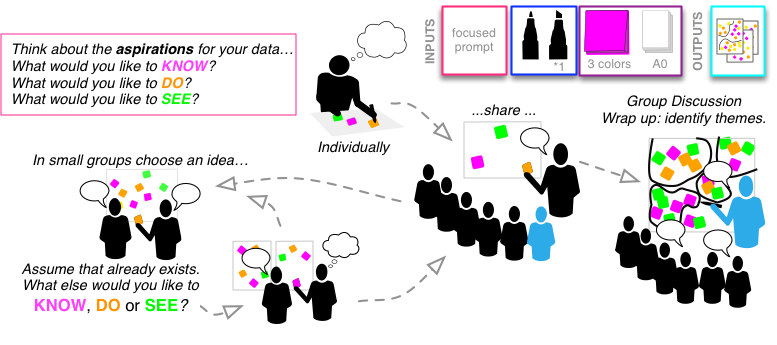
\includegraphics[width=\columnwidth]{figures/wishful-thinking-process}
    \caption{\sg{Placeholder - rehashed.. TBD what is needed = circles and divergence/convergence within method} \emph{Wishful Thinking} for Data Visualization Projects, adapted to ensure greater understanding of the needs and tasks of the application domain (to know, to do) and visual ideas (to see).}
     \label{fig:wishful-thinking-process}
\end{figure}

The \emph{wishful thinking} method in our example workshop (Fig.~\ref{fig:example-list}) is a visualization-specific form of \emph{aspirational thinking}~\cite{McFadzean1998b}. We have successfully used this method in a number of our workshops \ref{wor:eon}, \ref{wor:graffinity}, \ref{wor:cp}. Fig.~\ref{fig:wishful-thinking-process} illustrates the method in greater detail. 

The method starts with an individual activity with a low barrier to entry, which allows for a gentle step from opening into core. This, and then presenting the ideas to the room ensures inclusively, promotes \emph{agency} and can prompt the externalization of a wide range of ideas. To \emph{challenge} the participants the activities get progressively more difficult as participants form small groups and start to iterate and build upon these ideas by assuming that the initial idea has already been implemented [\ref{wor:eon},\ref{wor:cp}]. As an alternative we have also used hierarchical discussion from small group to large group discussion to explore interesting ideas [\ref{wor:graffinity}].

Whilst designing the workshop, an important input for this method is the focused scenario to which the method is being used. This must be adapted to the specific \emph{domain} \sg{?(as described in Sec.3.2)}. The participants are then asked to think about the scenario and answer the following questions: \emph{``What would you like to know? What would you like to see? What would you like to do?''}. These questions have been specifically formulated to adapt aspirational thinking to focus on \emph{data} and \emph{visualization}. 

We use different colored post-its for the externalization of ideas related to the three questions, as shown in Fig.~\ref{fig:wishful-thinking-process}. This encourages participants to create tangible artifacts, which can later be revisited, rearranged and used in our analysis. We have found the three questions prompt quite different responses and these are useful at different stages of the design process. \emph{``What do you want''}: \emph{``to do''} and \emph{``to know''} seem to be easier for the majority of participants to externalize. These ideas often refer to analytical tasks that they would like \emph{``to do''}, or envisaged insights they would like \emph{``to know''}.  \emph{``To see''} is often more of a \emph{challenge} for participants, but it ensures visualization appears early in the workshop. These initial ideas are then revisited and iterate as we build their visualization awareness and develop \emph{trust}. All three prompts can reveal unexpected or hidden goals. In addition to informing the design process, we have found that the \emph{``to know''} artifacts can formulate evaluative triggers for our prototype designs [\ref{wor:eon}].

\subsubsection{Visualization Analogies}

A second method that we have adapted is \emph{visualization analogies}, also in the example workshop (Fig.~\ref{fig:example-list}). This resembles analogy-based creativity methods~\cite{Gordon1961}. During \emph{visualization analogies} participants are shown a curated collection of visualizations. and \emph{challenged} to think (usually independently) about how aspects of the visualizations may apply to their domain. They are also asked to think about what they like and dislike about the visual examples. The diverse examples are important to prepare with care as they can not only result in increased \emph{interest} but also in the participant's \emph{trust} in researcher's domain expertise. Subsequent group discussions on these visualizations prompts \emph{collegiality} and increases \emph{agency}, and can result in some really inspiring ideas. 

Visualization analogies can inspire and engage participants while providing important domain information that can effectively inform ideas in ways that may inspire (diverge) and ground perspectives in visualization possibilities (converge). In this method, participants watch a presentation of curated visualizations while they are encouraged to think (usually individually) about what they like and dislike about the visualizations and how aspects of the visualizations may apply to their domain. The curated example visualizations will influence the workshop ideaspace. While the presentations used in the method will vary, we have presented a mix of examples with a range of objectives, including: those that we created (to show authority and credibility); those that we did not create (for diversity and to show knowledge of the field); older examples (to show depth of knowledge); challenging examples (to stretch thinking); playful examples (to support engagement and creativity); closely related examples (to make analogies easy); unrelated examples (to promote divergent thinking). Providing paper handouts that contain a representative image of each visualization enables participants to annotate, write down ideas or refer to specific visualizations [\ref{wor:graffinity},\ref{wor:cp},\ref{wor:arbor}].
%\reviseme{post-it notes are less effective for this method} [\ref{wor:eon}] \sg{is Eon the right ref? We didn't use post-its for this. Used blank paper for note taking. Changed for CP to structured page with prompts (the questions to think about with names of each example - no images) - so perhaps revise to 'relying solely on unstructured note taking is less effective for this method'}. 
The discussions during this method have expanded the workshop idea space in surprising ways, such as \emph{``what does it mean for legends to move?''} [\ref{wor:edina}], \emph{``what does it mean for energy to flow?''} [\ref{wor:eon}], and \emph{``what does it mean for neurons to rhyme?''}~[\ref{wor:graffinity}]. Although this method is primarily passive, participants report that it is engaging and inspiring to see the broad possibilities of visualization and relate them to their problems. It's an information-rich session that contains some new ideas and involves  directed activity. We postulate that this helps with the sharing of knowledge that is key to collaborative visualization design work and develops the levels of agency, ownership and authority that that are so important in collaborative design. Creativity workshops can foster and balance these feelings very effectively.

\sg{ I need to continue this description but I want to use context from 3.2 - so trying to get right content for each - help!}. 

\begin{figure}[t]
    \centering
    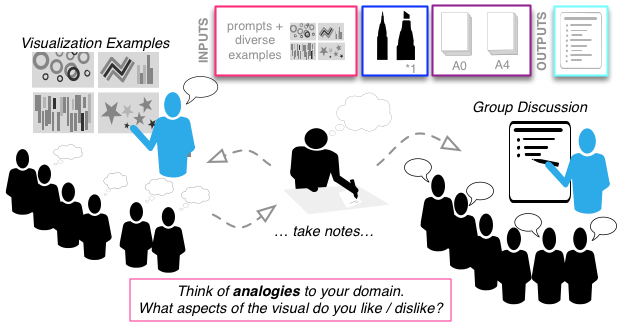
\includegraphics[width=\columnwidth]{figures/vis-aware-process}
    \caption{\sg{Placeholder} \emph{Visualization Analogies} for Data Visualization Projects.
    Passive presentation with individual ideation ensures inclusion and diversion. The group discussion results in some converging of ideas}
    \label{fig:vis-aware-process}
\end{figure}

\subsection{From Methods to Workshops}

\begin{figure}
    \centering
    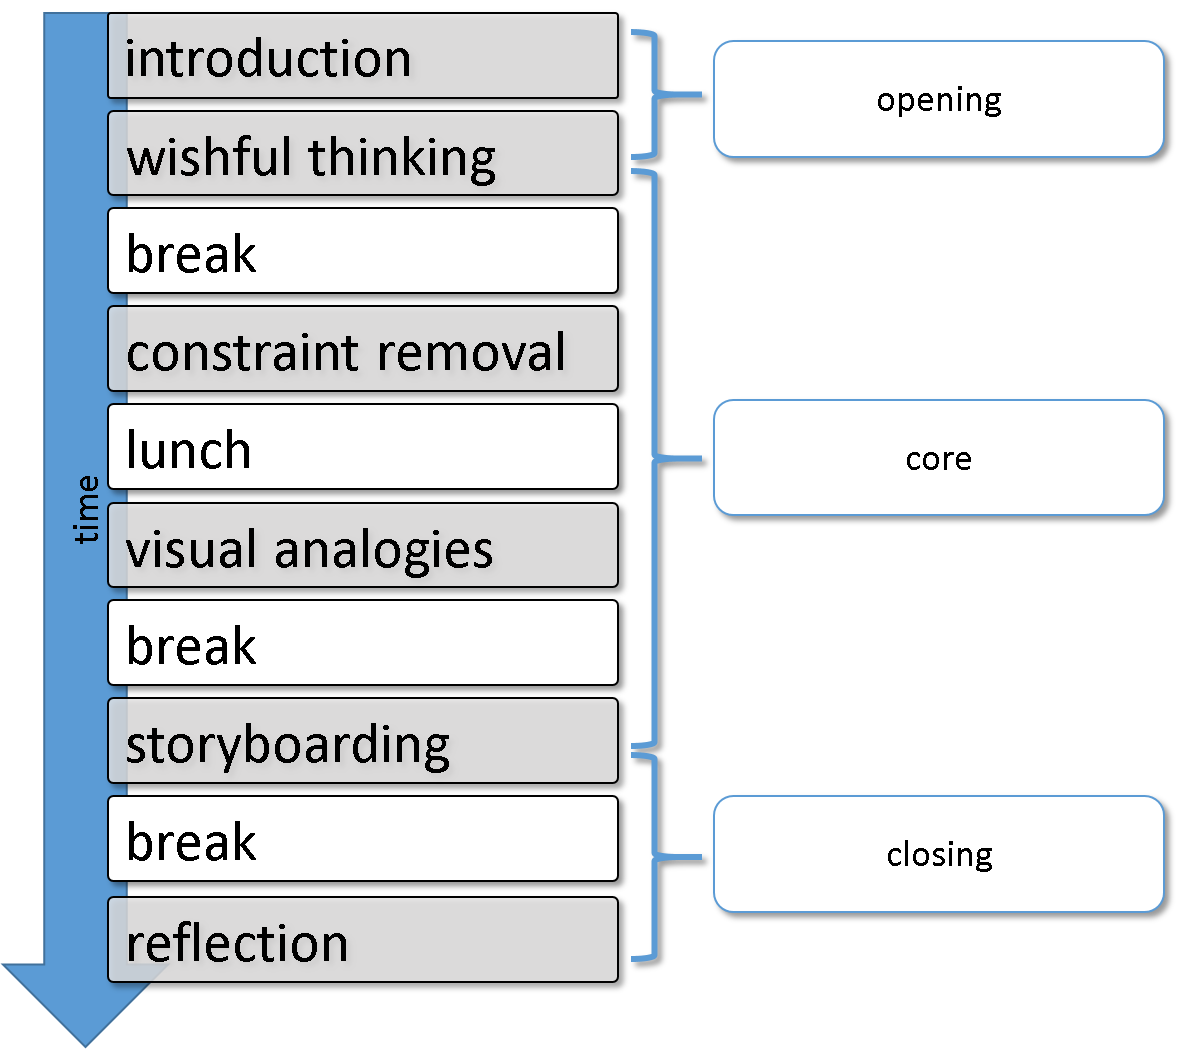
\includegraphics[width=\linewidth]{figures/example-list.png}
    \caption{\sg{EK's Placeholder! Something like this but it needs to be more connected to the text in the section - highlight the diverging, converging, incubation methods - perhaps with colour - also the data, vis, domain specific methods}}
    \label{fig:example-list}
\end{figure}

\ek{Frame creativity workshops as creativity support tools...use guidelines from creativity support tools~\cite{Shneiderman2005} to think about how to connect methods...}

First, selecting methods that \emph{``provide low barriers, high ceilings, wide walls''} is important as workshop participants should use their energy generating ideas instead of understanding methods (low barriers) and methods should allow for exploration without boundaries or stopping conditions (high ceilings and wide walls). We may want to \emph{challenge} participants to think broadly in places, but should ensure that they use their mental energy to think hard about the problem in hand and not to understand our methods.

In planning one workshop~[\ref{wor:eon}], we piloted a method in which ideas on post-it notes are placed on a drawing of a tree according to their implementation cost --- to discover low hanging fruit. We rejected this method as the initial activity in the workshop core because of its barriers, it required knowledge about the difficulty of ideas and resulted in discussion on implementation instead of the breadth of ideas. We deemed the barrier to entry to be too much of a \emph{challenge} that could result in a loss of  \emph{trust} and  \emph{interest}. 

Second, selecting methods to \emph{``support collaboration and communication''} underlies the entire purpose of the workshop. In our experience, every method that involves individual ideation is best balanced with group discussions to support the kinds of \emph{collegiality} that are typical of successful creativity workshops. Mixing groups between activities and ensuring that participants with different views, experiences and perspectives work together seems important. Our workshops often involve groups that are faceted on different criteria during different methods. Groups may grow through merging in hierarchical decision making processes~[\ref{wor:edina}].

Third, \emph{``invent things that you would want to use yourself''}. This advice has two dimensions in our experience. Firstly it is important that facilitators enjoy the activity, and we select methods that are playful, fun, engaging and productive. Running a workshop with methods that you know, trust and like to use will likely maintain the enthusiasm and energy of that you have as a workshop facilitator. Along with the use of relevant examples, efforts to ensure agency and direct variation of other factors (mix individual work with group work, limit high challenge activity - but introduce it in supportive ways and mix it with some low barrier work), this should maintain \emph{interest} in our experience. 


% \section{Design Model: Reflective Considerations} 
% \label{sec:design}

% This section introduces actionable design considerations, ideas that should be taken into account while selecting workshop methods,  fine-tuning existing workshops to a specific project and during a running a workshop. Summarized in Tab.~\ref{tab:design-considerations}, the considerations follow the three stages of the design model [\ref{des:context} -- \ref{des:action}] and provide guidance for selecting, and adapting workshop methods and reflecting on their use [\ref{des:resources} -- \ref{des:support}]. We support them with experiential details, relevant literature \new{and with reference to an illustrative example workshop outline that has been validated in three projects at three institutions [\ref{wor:eon},~\ref{wor:graffinity},~\ref{wor:cp}]. The six method, full day workshop shown in Fig.~\ref{fig:example-list} is described in greater detail in the Supplementary Material.}

% \subsection{Workshop Opening}

% The beginning of a workshop can be used to communicate the goals and guidelines for participants, but in our experience it is important that it is more than that --- it can dispel any assumptions that participation will be passive by encouraging self-expression, idea generation, open communication as well as establishing a safe co-owned environment in which creative contributions are valued. 
% It should be made clear that the workshop will be interesting, fun and useful.

% While participants should already know why they are attending the workshop (see Sec.~\ref{sec:recommendations}), the opening can reiterate the intended outcome --- often, the exploration of domain problems, visualization opportunities, and data analysis needs --- while establishing a shared context for participants and facilitators [\ref{des:context}]. We have opened workshops with a short introduction, summarizing the intended outcome with a \emph{``single indicative graphic''} [\ref{wor:edina}] or by posing a concise statement to frame the day as \emph{``guided activities that are meant to help us understand: what would you like to do with visualization?''}[\ref{wor:graffinity}]. Following existing methodologies~\cite{CreativeEducationFoundation2015,Osborn1953}, we have also introduced workshop guidelines to deliberately and explicitly support creativity, including [\ref{wor:eon}]:
% \begin{itemize}[noitemsep,nolistsep]
% \item all ideas are valid --- express them |\& record them;
% \item let everyone have their say; 
% \item be supportive of others; 
% \item instead of criticizing, create additional ideas;
% \item think `possibility' -- not implementation; 
% \item speak in headlines and follow-up with detail; and 
% \item switch off all electronic devices.
% \end{itemize}

% Keeping introductory presentations short can help to support creativity as we aim to encourage participants to generate ideas. Interpersonal introductions (i.e., \emph{icebreakers}) can be effective in the workshop opening as they encourage self-expression and risk taking, while potentially fostering trust and communication [\ref{des:interpersonal}]. One effective method, the \emph{analogy introduction}, asks facilitators and participants to introduce themselves through analogy, e.g., \emph{``if you were to describe yourself as an animal, what would you be?''} [\ref{wor:eon}]. Members of one academic lab with which we worked [\ref{wor:graffinity}], found this method particularly effective as it supported interpersonal leveling as everyone --- from undergraduates to senior researchers --- demonstrated vulnerability by expressing themselves. It's a good levelling technique which can help reinforce the views that \emph{all ideas are valid} and \emph{everyone can have their say}. Another effective opening method is \emph{visual improv}\footnote{A method where participants are asked to rapidly sketch increasingly complex objects, e.g., a line, a shape, a mountain, a pet, a mode of transportation, a dangerous mountain, a helpful pet, a friendly mode of transportation ... and then to quickly create a story from anyone's sketches and introduce themselves through the story.} as its pace necessitates suspending judgment and it potentially primes participants for thinking visually~\cite{Rogers2017}. We have also opened workshops with short introductions from participants and facilitators about their areas of research [\ref{wor:htva}]. However, more surprising and levelling introduction methods can help to establish an atmosphere conducive to creativity, particularly if participants work together regularly. Using analogy also primes participants for the type of thinking that is core to the visualization design process -- \emph{we could use this design for that task}.

% If the the workshop involves visualization researchers as well as domain collaborators, it may be useful for collaborators to summarize their domain challenges in the opening [\ref{des:leading}]. Collaborator led openings may increase engagement and senses of ownership and agency such as through presentations that: \emph{``describe [their challenges] as we establish data characteristics and analytic needs''} [\ref{wor:htva}]. But, this is not necessary in workshops where domain collaborators are the only participants. Passive methods, such as lectures and presentations, can discourage participation at the outset [\ref{des:beware}]. For example, one workshop started with a presentation on the current state of analysis tools [\ref{wor:arbor}], encouraging participants to passively listen rather than actively explore. We may need to vary levels of participation throughout a workshop, but the outset should be active and energized.    



% \begin{table}
    \small
    \centering
    \begin{tabular}{|m{0.07\linewidth}|p{0.8\linewidth}|}
    \hline
    ID & Consideration \\
    \hline
    \des{des:context}{} & Effective openings establish context and promote group creativity. \\
    \des{des:interpersonal}{} & Interpersonal introductions can support communication and creativity. \\
    \des{des:leading}{} & Allowing participants to lead in the opening may increase engagement. \\
    \des{des:beware}{} & Passive methods in the opening may discourage participation. \\
    \hline
    \des{des:ideaspace}{} & The ideaspace focuses on data, analysis, automation, and visualization.  \\
    \des{des:diverge-converge}{} & Diverge-converge cycles can develop the ideaspace.  \\
    \des{des:cascading}{} & Methods have cascading influences on the ideaspace.  \\
    \des{des:externalize}{} & Effective methods externalize ideas.  \\
    \des{des:post-it}{} & Post-it notes are particularly useful for externalization.  \\
    \des{des:passive}{} & Passive methods can support creativity.  \\
    \des{des:visualization-analogies}{} & Visualization analogies can excite and engage participants.  \\
    \des{des:convergence}{} & Convergence can conclude methods and the workshop core. \\
    \hline
    \des{des:closing}{} & Closing discussions can promote reflection and validation \\
    \des{des:feedback}{} & Effective closings can prepare participants to give feedback. \\ 
    \des{des:action}{} & Identifying the next steps of action can provide validation. \\
    \hline
%% JD \des{des:resources}{} & Existing resources describe a plethora of methods. \\
%% JD \des{des:tailor}{} & Methods can be tailored to explore visualization and data analysis. \\
%% JD \des{des:support}{} & Methods can be evaluated as creativity support tools.\\
    \des{des:resources}{} & Existing resources describe a plethora of methods. \\
    \des{des:select}{} & Methods should be selected in consideration of key characteristics (CACTI). \\
    \des{des:adapt}{} & Methods can be adapted to explore data, visualization and domain. \\
    \des{des:support}{} & Methods can be evaluated as creativity support tools.\\

    \hline
    \end{tabular}
    \caption{Summary of the workshop design considerations.}
    \label{tab:design-considerations}
\end{table}


% \begin{figure}
%     \centering
%     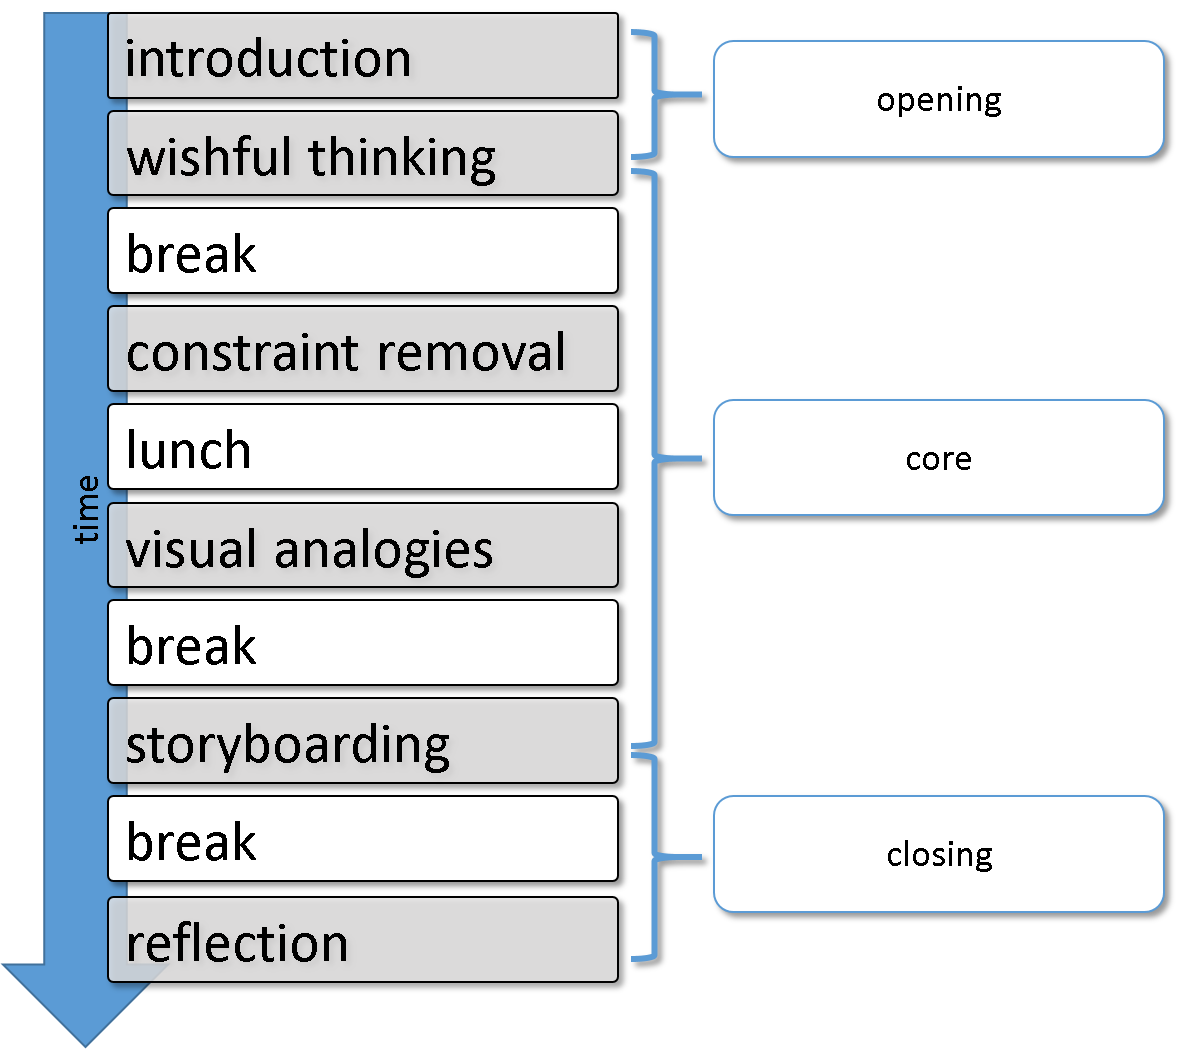
\includegraphics[width=\linewidth]{figures/example-list.png}
%     \caption{\sg{EK's Placeholder! Something like this but it needs to be more connected to the text in the section - highlight the diverging, converging, incubation methods - perhaps with colour - also the data, vis, domain specific methods}}
%     \label{fig:example-list}
% \end{figure}

% \subsection{Workshop Core}

% While an effective opening establishes a creative mindset, the core harnesses that mindset to explore relevant ideas. It can appear chaotic as participants audaciously ideate, creating hundreds of post-it notes or other artifacts. Yet, common considerations underlie effective cores.

% The workshop \emph{ideaspace}, the abstract set of all ideas currently being considered~\cite{Biskjaer2017}, typically focuses on relevant domain challenges, data, analysis tools, automation, and visualization [\ref{des:ideaspace}]. The ideaspace is established through methods that ask participants to think creatively about these topics. Inline with the design study methodology~\cite{Sedlmair2012}, we select methods that focus on analysis needs as opposed to potential solutions. For example, we have asked participants about the good and bad aspects their current workflows~[\ref{wor:htva}], instead of directly asking for envisioned solutions. Moreover, we use methods that ask a variety of questions, approaching analysis needs from different perspectives, to encourage the sharing of tacit knowledge. Knowledge sharing and task clarification enables us to differentiate between tasks that can be automated and those that might benefit from visualization and provide opportunities for learning about it (see \cite{Sedlmair2012} Fig.~1.). 

% Workshop methods can be characterized by their influence on the ideaspace. \emph{Divergent} methods expand the ideaspace, while \emph{convergent} methods contract it~\cite{Osborn1953}. Diverge-converge cycles can explore a broad ideaspace and then winnow it to the more interesting ideas, which are often outside the initial ideaspace [\ref{des:diverge-converge}]. Diverge-converge cycles can occur within methods, such as in an example of \emph{brainstorming}~\cite{Osborn1953}, in which participants record \emph{``problems and successes associated with the current clients on sticky notes''} and then share the more interesting ideas [\ref{wor:edina}]. Diverge-converge cycles can also occur between methods, as in the same workshop [\ref{wor:edina}], where the ideaspace diverged from current problems and successes, to aspirations for future software, and subsequently converged to specific visualization tasks.
% This may be particularly important where domain experts are solution focussed and involved in creative activity. In our work on visualization map legends [\ref{wor:edina}] developers who were focussed on implementing solutions within given technology participated in the workshop. Aspirational thinking exercises were used to create design targets that involved more general characteristics than those proposed in the original discussion: 
% `\emph{It is so beautiful, I want to put it on the wall}',
% `\emph{I have the map I wanted in less than a minute}',
% `\emph{The legend could tell me at a glance what was on the map}'.
% Subsequent exercises, both within this workshop and at subsequent creative events, enabled us to ground these ideas, develop tasks around them and establish priorities.   
% Diverge-converge cycles occur in all of our workshops and we have planned and experienced them at a range of scales from within-method (e.g.~Figs.~\ref{fig:wishful-thinking-process}~\&~\ref{fig:vis-aware-process}) to between-workshop. Such cycles are illustrated in our example workshop in ~Fig.\ref{fig:example-list} 

% When used early in the core, divergent methods generate ideas that propagate through the workshop [\ref{des:cascading}], and the methods can be fine-tuned to explore relevant topics. Consider \emph{wishful thinking} \new{the second method in our example workshop (Fig.~\ref{fig:example-list})}, where participants are prompted with a domain-specific scenario. %respond to the following questions on post-it notes: \emph{``What would you like to know? What would you like to see? What would you like to do?''}
% For example, in a collaboration to explore long term goals for emerging technology~[\ref{wor:eon}], we asked participants to think about their \emph{``aspirations for the SmartHome programme...''}, which generated forward-thinking ideas about energy consumption, such as to better understand \emph{``the value of the data.''} In collaborations to explore current analysis needs, we asked  neuroscientists~[\ref{wor:graffinity}], \emph{``suppose you are analyzing a connectome...''} and constraint programmers~[\ref{wor:cp}], \emph{''your program does not execute as expected...''} Participant responses revealed shorter term goals, to \emph{``to understand neuron connectivity''} and to \emph{``explore the [solver] search space,''} respectively.
% \\
% \jd{@EK -- see my comment on the flow problem here ...}\\

% %\emph{Wishful thinking} is an example method that encourages participants to externalize ideas by creating tangible artifacts. \sg{link forward: The method is explained in greater depth in sec.5.4?} 
% Selecting methods that externalize ideas, such as \emph{wishful thinking}, supports workshop analysis as visualization researchers discover domain challenges and visualization opportunities expressed in the artifacts [\ref{des:externalize}]. Externalization can encourage creative thinking, as physically expressing an idea forces the creator to elaborate and improve it~\cite{Sawyer2006}.
% \jd{This is so important, and links so nicely to analysis, that I would like to extend [\ref{des:externalize}] to say something like -- ``Effective methods externalize \emph{and analyse} ideas'', which covers ranking, grouping, etc and prepares analysts for R13 and R14. In fact, given the next paragraph, [\ref{des:post-it}] this could be extended to say ``Post-it notes are particularly useful for externalization and (preliminary) analysis''.}
% And, artifacts enable communication between group members, as ideas are moved, ranked or aggregated. Materials that are effective for externalizing ideas include whiteboards for \emph{brainstorming}, or butcher paper for \emph{visual improv}. 

% Post-it notes are a particularly useful form of externalization that we have used in all of our requirements workshops [\ref{des:post-it}]. The critical role of post-it notes to support communication and both divergence and convergence has been described by design researchers as~\cite{Dove2016}: \emph{``post-it notes are grouped with reference to the emergence of specific concepts and themes ... through this grouping they `evolve' into more complex forms ... they are used as objects to think with, and ... they support a common understanding of the work at hand''}. In our experience, the grouping or revisiting of concepts on post-it notes supports emerging themes that represent domain challenges. Using post-it note color to encode information, such as the method or specific prompt that generated an idea, can provide insight structure to the method, help with recording and be a useful aid during analysis as it can establish how ideas evolved and were valued through the workshop [\ref{des:externalize}], [\ref{des:post-it}] \jd{And \ref{rec:artifacts}, but we are not talking about that yet?!}. 

% As continuously generating ideas can tire participants, passive methods can be added to the core to provide  some variation to a workshop and support creativity by providing time for incubation [\ref{des:passive}], the conscious and unconscious combination of ideas~\cite{Sawyer2006}. Incubation can be supported through unstructured breaks between methods, or informal discussions over meals\new{, as shown in the example workshop outline (Fig.~\ref{fig:example-list})}. It can also be supported through the use of passive methods, such as, those that encourage participants to listen to presentations. Asking participants to reflect upon their contents, record reactions or perhaps to produce structured notes provides some focus and interest to passive activity that can be informative, varies pace and allows time for incubation. We have typically used passive methods in the second half of full day workshops, to provide incubation after lunch [\ref{wor:eon},~\ref{wor:graffinity},~\ref{wor:cp},~\ref{wor:arbor}].

% The example workshop  (Fig.~\ref{fig:example-list}) outlines a passive method after lunch that we have developed for the visualization domain. Visualization analogies can \new{inspire} and engage participants while providing important domain information that can effectively inform ideas in ways that may inspire (diverge) and ground perspectives in visualization possibilities (converge) [\ref{des:visualization-analogies}].
% In this method, participants watch a presentation of curated visualizations while they are encouraged to think (usually individually) about what they like and dislike about the visualizations and how aspects of the visualizations may apply to their domain. The curated example visualizations will influence the workshop ideaspace. While the presentations used in the method will vary, we have presented a mix of examples with a range of objectives, including: those that we created (to show authority and credibility); those that we did not create (for diversity and to show knowledge of the field); older examples (to show depth of knowledge); challenging examples (to stretch thinking); playful examples (to support engagement and creativity); closely related examples (to make analogies easy); unrelated examples (to promote divergent thinking). Providing paper handouts that contain a representative image of each visualization enables participants to annotate, write down ideas or refer to specific visualizations [\ref{wor:graffinity},\ref{wor:cp},\ref{wor:arbor}].
% %\reviseme{post-it notes are less effective for this method} [\ref{wor:eon}] \sg{is Eon the right ref? We didn't use post-its for this. Used blank paper for note taking. Changed for CP to structured page with prompts (the questions to think about with names of each example - no images) - so perhaps revise to 'relying solely on unstructured note taking is less effective for this method'}. 
% The discussions during this method have expanded the workshop idea space in surprising ways, such as \emph{``what does it mean for legends to move?''} [\ref{wor:edina}], \emph{``what does it mean for energy to flow?''} [\ref{wor:eon}], and \emph{``what does it mean for neurons to rhyme?''}~[\ref{wor:graffinity}]. Although this method is primarily passive, participants report that it is engaging and inspiring to see the broad possibilities of visualization and relate them to their problems. It's an information-rich session that contains some new ideas and involves  directed activity. We postulate that this helps with the sharing of knowledge that is key to collaborative visualization design work and develops the levels of agency, ownership and authority that that are so important in collaborative design. Creativity workshops can foster and balance these feelings very effectively.

% While these  methods tend to expand the ideaspace, convergent discussions can be used to conclude individual methods and convergent methods are an important way of concluding the workshop core as the structuring that occurs makes the outputs of this activity more manageable [\ref{des:convergence}]. Individual methods can be concluded with the sharing of ideas that are deemed interesting, exciting, or potentially influential. These discussions can reinforce the importance of open communication and exploration throughout the workshop. Similarly, the workshop core can conclude with methods that are designed to group, rank, or summarize ideas from the day. In our two day workshop, we concluded the first day by clustering ideas to identify \emph{springboards}~\cite{Gordon1961}, that we explored during the second day [\ref{wor:arbor}]. We have used \emph{storyboarding}\new{, as shown in the example workshop (Fig.~\ref{fig:example-list}),} to encourage the synthesis of ideas into a single narrative [\ref{wor:eon}, \ref{wor:graffinity} \ref{wor:cp}]. This can be used to winnow ideas into useful and foreseeable opportunities where participants for example depict \emph{`a day in the life'} imagining the impact of having implemented ideas from the workshop in their work place.  We have also asked participants to explicitly rank ideas, providing cues for analyzing the workshop results [\ref{wor:eon},~\ref{wor:htva}]. \sg{we didn't in P2.R but did in P2.D2 - can we refer to this?} Regardless of the method used, the core of every workshop in our experience transitions to the closing with convergent methods.

% \jd{Perhaps there is something missing here that refers to either: i) a visualization specific output (graphic -- sketch or annotated examples from vis awareness) at the end of the core? or, ii) use of a vis process model in convergent activity - e.g. DSM Fig 1 - what are the tasks for which VIS could apply? DAF?}
% \sg{Yes JD let's discuss. I think the amount of visual output also depends on the ratio of vis to collaborators as participants. And to a degree the number of participants (i.e. was less easy with the small eon group). An idea I discussed with SJ and GD pre-CP was to improve on storyboards by getting vis experts in to partner up with collaborators to create quick visual ideas - this was too difficult for us logistically so we didn't but had we had vis participants there all/most of the day we could have easily done some form of speed sketching} 
% \jd{I certainly think we need to say this somewhere -- this is part of the \emph{how do we adapt and why?} discussion}  

% \subsection{Workshop Closing}
% \label{Workshop Closing}

% The end of the workshop is an opportunity to reflect on the shared creative experience, to validate the time and energy that participants have contributed, and to identify the next steps of action.

% Discussions during the closing can promote reflection, potentially providing validation to participants and generating information valuable for workshop analysis [\ref{des:closing}]. Encouraging participants to reflect on how their ideas have evolved, such as by asking, \emph{``what do you know now that you did not know this morning?''} [\ref{wor:eon}] or ,\emph{''what will you do differently tomorrow given what you have learned today?''} [\ref{wor:cp}] can provide validation for the time committed to the workshop. One participant, for example, reported \emph{``I was surprised by how much overlap there was with the challenges I face in my own work and those faced by others''} [\ref{wor:cp}]. Also, because reflective questions are used to start a discussion, they require participants to rank their thoughts and to talk about the more interesting ones. Recording these ideas can provide important clues for the analysis of workshop artifacts, such as in our neuroscience workshop's concluding where discussions about \emph{``multi-hop path queries''} resulted in focusing on connectivity analysis [\ref{wor:graffinity}].

% Effective closings can prepare participants to provide feedback on their experiences [\ref{des:feedback}]. Analyzing feedback enables the workshop team to reflect on the execution and the efficacy of specific methods. Although we have tried gathering feedback in a low-cost way that has been suggested for enabling post-workshop incubation, by handing out stamped postcards for participants to mail back to us, the number of responses was underwhelming [\ref{wor:eon}]. Recently, we have used online surveys to gather feedback on the effectiveness of the workshop, specific methods, and the facilitation style. While the closing is an appropriate time to ask for feedback, responses to online surveys can be spread over days and may require additional reminders. We have asked participants for feedback during the workshop [\ref{wor:eon}], but do not yet understand how providing time for incubation or enabling anonymous responses influences the results.

% Lastly, identifying the next steps of action can validate participant involvement, as the workshop team can explain how the ideas will be used to move the collaboration forward [\ref{des:action}] --- this includes any post-session feedback, but also the analysis and action planned, as we describe in Sec.~\ref{sec:recommendations}.  

% \subsection{Workshop Methods -- Factors for Consideration}

% \jd{or ... \textbf{adoption}}\\
% %\sg{we need to say something about characterized methods and that we can not describe the best workshop - as this depends entirely on the problem, the participants, the facilitators, constraints (where did these go are they still in the paper) etc but in this paper we do provide the building blocks to support researchers to understand and develop their own workshops and workshop methods in order to run successful and creative workshops in the future..} \jd{I try to address this below - may need re-writing a bit} \\

% These design considerations are intended as prompts for thinking about workshops when selecting from the range of creativity techniques for appropriate methods to \textbf{adopt}. As such, they provide a useful overview for planning.
% But the way in which methods are used will depend upon the details and the dynamics of the workshop, and there is plenty of scope for variation in both cases.
% We have found it useful to plan and run methods  by considering a small number of key factors for the workshop and its participants: 
% %% they are also a number of method mechanics, that are important to vary throughout the workshop to ensure that we engage, educate and learn from our participants.
% %% These method mechanics are shown in Table ??.
% %%
% the scope for achieving and varying levels of \emph{collegiality}, \emph{agency}, \emph{challenge}, \emph{trust} and \emph{interest} associated with each.
% These have been important factors associated with likely workshop success in our experience. To help us remember the five we term them \textbf{CACTI} \emph{factors}. Each creativity method offers particular opportunities to vary levels of these factors that need to be managed throughout a workshop along with levels of engagement with data, visualization and the specialist domain in which collaborators are working. 
% The degree to which each method delivers what is intended is somewhat unpredictable.
% This is the case in terms of direct outputs, but also indirect effects on the key factors that can result in a productive and creative  workshop.

% \begin{itemize}[noitemsep,nolistsep]
% \item\textbf{C}~ollegiality -- the degree to which communication and collaboration are encouraged and occur;
% \item\textbf{A}~gency -- the sense of participant ownership in workshop outcomes (and perhaps process);
% \item\textbf{C}~hallenge -- the barrier of entry to, and likelihood of success in workshop methods and tasks; 
% \item\textbf{T}~rust --  the confidence that participants have in the methods, the design process and in the researcher's domain expertise; 
% \item\textbf{I}~nterest -- the amount of attention, energy and engagement that occurs;
% \item\textbf{+}~ -- other \emph{relevance} factors that can effect these: \\the levels of engagement with \emph{data}, \emph{visualization} and the specialist \emph{domain} in which collaborators are working.
% \end{itemize}


% %% C -- this includes ensuring all participants are included at all times
% %% C -- ensures the appropriate difficultly of the workshop methods and tasks

% The factors are not independent, neither are they consistent or easily measurable. They do not map exactly to particular methods and the extent to which the various methods enable and effect them will depend upon who uses them, how, in what contexts and various (often unknown and unpredictable) characteristics of the workshop group.
% And yet maintaining appropriate levels of collegiality, agency, challenge, trust, interest and domain focus are likely to be important if workshops are to be inspiring and enjoyable.
% \jd{cite Shneiderman(?) on enjoyable?}
% Enjoyable workshops, are not only more likely to produce valuable outputs in our experience, but are likely to establish lasting rapport and build trust among researchers and collaborators.  

% Creating a workshop plan that builds and moderates these characteristics is of course as much of a craft as design itself. As is responding to a failing method (\emph{nobody feels like an animal this morning}; \emph{post-its don't stick}), a loss of interest (\emph{there is no energy}; \emph{the room is too hot}; \emph{we had a tough away day yesterday}) or a lack of agency (\emph{some participants dominate some tasks}).
% Given our collective experience, we offer some examples of methods in action that show how they have worked and failed in light of these 5 factors\. These considered experiences could be informative and instructive in pre-workshop planning and in the essential on-the-fly workshop management that is required for a successful event.


% Framing workshops as \emph{creativity support tools} can provide criteria to select effective methods [\ref{des:support}]. While all of the creativity support tool guidelines proposed by Shneiderman et al.~\cite{Shneiderman2005} are valuable to workshop design,
% %% three seem particularly relevant given our experiences. 
% three seem to relate closely to the factors we have identified.

% First, selecting methods that \emph{``provide low barriers, high ceilings, wide walls''} is important as workshop participants should use their energy generating ideas instead of understanding methods (low barriers) and methods should allow for exploration without boundaries or stopping conditions (high ceilings and wide walls). We may want to \emph{challenge} participants to think broadly in places, but should ensure that they use their mental energy to think hard about the problem in hand and not to understand our methods.

% In planning one workshop~[\ref{wor:eon}], we piloted a method in which ideas on post-it notes are placed on a drawing of a tree according to their implementation cost --- to discover low hanging fruit. We rejected this method as the initial activity in the workshop core because of its barriers, it required knowledge about the difficulty of ideas and resulted in discussion on implementation instead of the breadth of ideas. We deemed the barrier to entry to be too much of a \emph{challenge} that could result in a loss of  \emph{trust} and  \emph{interest}. 

% Second, selecting methods to \emph{``support collaboration and communication''} underlies the entire purpose of the workshop. In our experience, every method that involves individual ideation is best balanced with group discussions to support the kinds of \emph{collegiality} that are typical of successful creativity workshops. Mixing groups between activities and ensuring that participants with different views, experiences and perspectives work together seems important. Our workshops often involve groups that are faceted on different criteria during different methods. Groups may grow through merging in hierarchical decision making processes~[\ref{wor:edina}].

% \sg{@EK can you add the missing citations and proj, a lot of this text was taken from your google doc}
% This incorporates the need to establish \emph{agency} -- the feeling of ownership, responsibility, and ability to act~\cite{Brooks-Harris1999} promoted by using methods that encourage multi-directional communication between workshop participants and facilitators~\cite{Brooks-Harris1999}. Methods that encourage one-way communication, such as lectures, are notorious for hindering agency ~\cite{Lloyd2011}. Yet, this is a mistake we have made [P8].  Establishing \emph{Trust} is an important factor and must be achieved initially and reinforced if collaboration is to be successful and communication is to work well. Trust is the confidence that participants place in each other and in the workshop team. Encouraging trust between participants and facilitators leads to open communication, the uninhibited sharing of ideas between individuals [Jones1989]. This can be achieved by showing intent to listen, and demonstrating vulnerability ~\cite{Brooks-Harris1999}.
% Achieving trust in the process (see opening), the knowledge of the academic experts, the value of participants' knowledge (see agency) and the  likely impact of the day's activities (see closing) are all important and can be achieved in a number of ways. The visualization awareness exercise can be used to show the breadth of knowledge of the visualization specialists, and situate their contributions to the academic discipline. On occasion we have trusted participants to lead sessions or fix technology problems that have occurred.

% Following one workshop in which we evidently achieved academic credibility, senior analysts were more willing to spend time with us answering our domain questions, discussing their needs, and evaluating prototypes. 

% Third, \emph{``invent things that you would want to use yourself''}. 
% This advice has two dimensions in our experience. Firstly it is important that facilitators enjoy the activity. So adopt methods that are playful, fun, engaging and productive. Workshop methods can be selected from a growing body of valuable resources [\ref{des:resources}] and should always be tested in advance.
% Running a workshop with methods that you know, trust and like to use will likely maintain the enthusiasm and energy of that you have as a workshop facilitator.
% Along with the use of relevant examples, efforts to ensure agency and direct variation of other factors (mix individual work with group work, limit high challenge activity - but introduce it in supportive ways and mix it with some low barrier work), this should maintain \emph{interest} in our experience. 

% We have used methods from the following resources: McKenna et al.~\cite{McKenna2014}, who provide 100 exemplar methods relevant for visualization researchers, but these methods may need to be adapted to a workshop setting; Kumar~\cite{Kumar2012}, who describes 101 product design methods useful in a business setting; Gray et al.~\cite{Macanufo2010}, who describe methods that encourage creative thinking and can be chained together into workshops.We have also drawn inspiration from Tinkertoys~\cite{Michalko2006}, which describes creative-thinking techniques to approach and solve problems at home and in business; as well as Innovation Games~\cite{Hohmann2007} and Game Storming~\cite{Macanufo2010}, which both describe methods in the form of innovative games for improving workplace engagement, idea generation and communication. \sg{In addition, there are online references such as \url{https://www.mycoted.com/Category:Creativity_Techniques} and \url{http://becreative.city.ac.uk/} where established creativity techniques are characterizes by criteria. Perhaps some of these could be added / listed as footnotes - check with SJ as how useful?}.
% Knowing these resources and finding alternatives as they emerge, adopting methods in light of likely effects on \emph{CACTI} factors, and logging experiences are important components of creative visualization workshop design.


% %% JD -- It is particularly important as we look to incorporate data, visualization and the application domain into the workshop methods. 


% \subsection{Workshop Methods -- Data, Visualization~\& Domain}
% \jd{or ... \textbf{adaption}}\\

% The majority of these resources target domains outside of visualization, but we see plenty of scope for \textbf{adapting} established creativity methods for use in visualization design and have some experience of this working effectively.
% Being creative in this way allows us to engage with meaningful \emph{data}, through \emph{visualization} and tailor workshops to the specialist \emph{domain}. In turn, this can achieve \emph{trust} and \emph{agency} and develop and maintain \emph{interest}.
% It is achieved by injecting vocabulary, imagery and technology to explicitly focus on domain challenges, data characteristics, visual methods or analysis tasks [\ref{des:adapt}]. In the following section we present some of our adapted methods.

% The \emph{wishful thinking} method in our example workshop (Fig.~\ref{fig:example-list}) is a visualization-specific form of \emph{aspirational thinking}~\cite{McFadzean1998b}. We have successfully used this method in a number of our workshops \ref{wor:eon}, \ref{wor:graffinity}, \ref{wor:cp}. Fig.~\ref{fig:wishful-thinking-process} illustrates the method in greater detail. 

% The method starts with an individual activity with a low barrier to entry, which allows for a gentle step from opening into core. This, and then presenting the ideas to the room ensures inclusively, promotes \emph{agency} and can prompt the externalization of a wide range of ideas. To \emph{challenge} the participants the activities get progressively more difficult as participants form small groups and start to iterate and build upon these ideas by assuming that the initial idea has already been implemented [\ref{wor:eon},\ref{wor:cp}]. As an alternative we have also used hierarchical discussion from small group to large group discussion to explore interesting ideas [\ref{wor:graffinity}].


% Whilst designing the workshop, an important input for this method is the focused scenario to which the method is targetted. This must be adapted to the specific \emph{domain} \sg{?(as described in Sec.3.2)}. The participants are then asked to think about the scenario and answer the following questions: \emph{``What would you like to know? What would you like to see? What would you like to do?''}. These questions have been specifically formulated to adapt aspirational thinking to focus on \emph{data} and \emph{visualization}. 

%  \begin{figure}[t]
%      \centering
%      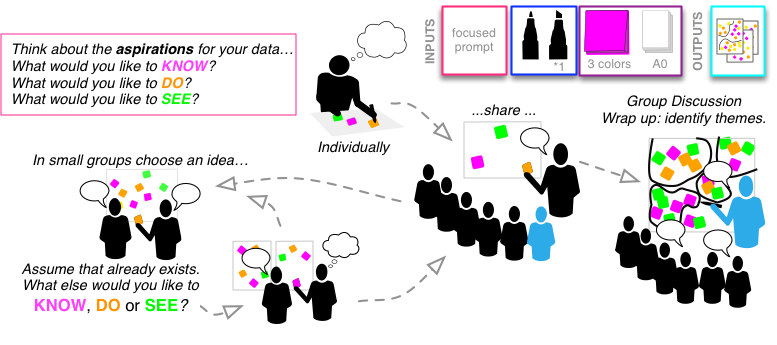
\includegraphics[width=\columnwidth]{figures/wishful-thinking-process}
%      \caption{\sg{Placeholder - rehashed.. TBD what is needed = circles and divergence/convergence within method} \emph{Wishful Thinking} for Data Visualization Projects, adapted to ensure greater understanding of the needs and tasks of the application domain (to know, to do) and visual ideas (to see).}
%      \label{fig:wishful-thinking-process}
%  \end{figure}

% We use different colored post-its for the externalization of ideas related to the three questions, as shown in Fig.~\ref{fig:wishful-thinking-process} [\ref{des:externalize}, \ref{des:post-it}]. This encourages participants to create tangible artifacts, which can later be revisited, rearranged and used in our analysis. We have found the three questions prompt quite different responses and these are useful at different stages of the design process. \emph{``What do you want''}: \emph{``to do''} and \emph{``to know''} seem to be easier for the majority of participants to externalize. These ideas often refer to analytical tasks that they would like \emph{``to do''}, or envisaged insights they would like \emph{``to know''}.  \emph{``To see''} is often more of a \emph{challenge} for participants, but it ensures visualization appears early in the workshop. These initial ideas are then revisited and iterate as we build their visualization awareness and develop \emph{trust}. All three prompts can reveal unexpected or hidden goals. In addition to informing the design process, we have found that the \emph{``to know''} artifacts can formulate evaluative triggers for our prototype designs [\ref{wor:eon}].

% A second method that we have adapted is \emph{visualization analogies}, also in the example workshop (Fig.~\ref{fig:example-list}). This resembles analogy-based creativity methods~\cite{Gordon1961}. During \emph{visualization analogies} participants are shown a curated collection of visualizations. and \emph{challenged} to think (usually independently) about how aspects of the visualizations may apply to their domain. They are also asked to think about what they like and dislike about the visual examples. The diverse examples are important to prepare with care as they can not only result in increased \emph{interest} but also in the participant's \emph{trust} in researcher's domain expertise. Subsequent group discussions on these visualizations prompts \emph{collegiality} and increases \emph{agency}, and can result in some really inspiring ideas. 

% \sg{ I need to continue this description but I want to use context from 3.2 - so trying to get right content for each - help!}. 



 
%  \begin{figure}[t]
%      \centering
%      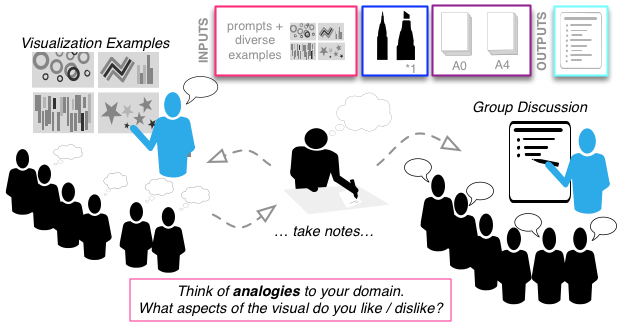
\includegraphics[width=\columnwidth]{figures/vis-aware-process}
%      \caption{\sg{Placeholder} \emph{Visualization Analogies} for Data Visualization Projects.
%      Passive presentation with individual ideation ensures inclusion and diversion. The group discussion results in some converging of ideas}
%      \label{fig:vis-aware-process}
%  \end{figure}

% \jd{The following may or may not be subsections - but I am adding them for now as candidates to show intended structure}

% \subsubsection{Real Data}
% \jd{Examples where we use real data - eg. E.ON, EDINA, HDVA?. CUrrently this requires \emph{time} and multiple workshops, but I want to say something in here about speeding up development cycles.}

% \subsubsection{Interactive Visualization}
% \jd{Have we ever used interactive visualization in a workshop?}

% \subsubsection{Early Data Vis}
% In our experience, data and visualization should be introduced to the design process early.\\
% \jd{Here is where we could talk about JD workshops being organized in a series giving time for development work -- and perhaps even possibly think about ways of speeding things up that have developed since. I like the idea of doing some thinking here based on ways of getting data and vis (including interaction) into the workshop early. Sorry it has not happened yet.}

% For the continued evolution of creativity workshops within applied visualization projects we see plenty of scope for adapting and incorporating other creativity methods [e.g. ..... fill some in here....]\\
% \jd{Something I can think about} in ways that use graphics as both stimuli and outputs.

% \sg{there is still work needed here but getting there}

% % \subsection{Design Resources}

% % The design considerations are tools for thinking about workshops from an overview-to-details, and provide a template for the design of future workshops. For example, we can select introductory methods for the opening; plan divergent, passive, and convergent methods for the core; and use reflective discussions for the closing. 

% % Workshop methods can be selected from valuable existing resources [\ref{des:resources}]. We have used methods from the following resources: McKenna et al.~\cite{McKenna2014} provide 100 exemplar methods relevant for visualization researchers, but these methods may need to be adapted to a workshop setting; Kumar~\cite{Kumar2012} describes 101 product design methods useful in a business setting; and Gray et al.~\cite{Macanufo2010} describe methods that encourage creative thinking and can be chained together into workshops. \sg{It sounds like we only used these three? We used Tinkertoys (M.Michalko) and Innovation Games (L.Hohmann) for Eon (and CP) ws design as referenced in ~\cite{Goodwin2013} - again outside vis domain but targetting workshops and creativity} All but one of these resources were targeted for domains outside of visualization and the methods should be adapted for visualization design by injecting vocabulary to explicitly ask about domain challenges, data characteristics, or analysis tasks [\ref{des:tailor}]. For example, \emph{wishful thinking} method which is a visualization-specific form of \emph{aspirational thinking}~\cite{McFadzean1998b}. Another tailored example is \emph{visualization analogies}, which resembles analogy-based creativity methods~\cite{Gordon1961}. We see plenty of scope for adapting such methods in ways that use graphics as both stimuli and outputs. \sg{I'd forgotten wishful thinking and vis analogies were described in 5.2.- can we refer back or forward to sec. 6 here or reference the workshops when they were run to show experience? currently these names seem to appear without any context. It is also not very clear if we tailored (and piloted) these ourselves rather than taking direct from the references - perhaps we need to be more explicit?}

% % Framing workshops as \emph{creativity support tools} can provide criteria to select effective methods [\ref{des:support}]. While all of the creativity support tool guidelines proposed by Shneiderman et al.~\cite{Shneiderman2005} are valuable to workshop design, three effectively describe our experience. First, selecting methods that \emph{``provide low barriers, high ceilings, wide walls''} is important as workshop participants should use their energy generating ideas instead of understanding methods (low barriers) and methods should allow for exploration without boundaries or stopping conditions (high ceilings and wide walls). In planning one workshop~[\ref{wor:eon}], we \new{piloted} \rem{considered} a method in which \new{ideas on} post-it notes are placed on a drawing of a tree according to their implementation cost --- to discover low hanging fruit. We rejected this method because of its barriers, it required knowledge about the difficulty of ideas and \new{resulted in discussions about implementation rather than the innovation of the ideas} \rem{putting fruit onto a tree was potentially confusing}. \sg{i.e. we got stuck in the detail} Second, selecting methods to \emph{``support collaboration and communication''} is the entire purpose of the workshop. In our experience, every method that involves individual ideation is balanced with group discussions. Third, \emph{``invent things that you would want to use yourself''} by creating methods that are playful, fun, engaging and productive. In addition to creating valuable output that expresses domain challenges and analysis tasks, enjoyable workshops can help to establish rapport and build trust among researchers and collaborators. \ek{Not sure if this paragraph makes sense.}
% % \jd{Yes -- I like it. I think it could be improved if we had an explicit link to the list of things we are trying to achieve somewhere: agency, collaboration, etc. This was the idea I had about the characteristics that we were trying to promote (SG worked on this?). But this is not necessary. It's OK without, this is just an opportunity to add a little more internal linking / structure. OK without!}
% % -----------------------------------------------------
% % -----------------------------------------------------

% % \begin{itemize}[noitemsep,nolistsep]
% % \item  \emph{Support collaboration and communication} --- workshops support communication by encouraging group work and explicitly externalizing ideas.
% % \item  \emph{Provide low barriers, high ceilings, wide walls} --- workshops encourage exploration through easy-to-use methods and undefined stopping conditions.
% % \item  \emph{Make it as simple as possible} --- workshops focus participant energy on the ideas, instead of understanding the method.
% % \item  \emph{Invent things that you want to use yourself} --- workshops use methods that are fun and engaging.
% % \item \emph{Support many paths and many styles} --- workshops support the different styles and preferences of participants.
% % \end{itemize}
% % Combining these guidelines with the workshop structure provide a foundation for selecting methods for creativity workshops.
% % \jd{Sure, but we are a little shor of examples that show that we have used these criteria in our selection}.




% % \begin{table}
    \small
    \centering
    \begin{tabular}{|m{0.7\linewidth}|m{0.03\linewidth}|m{0.03\linewidth}|m{0.03\linewidth}|}
        \hline
        \textbf{Method Characteristics} & \textbf{Op.} & \textbf{Co.} & \textbf{Cl.} \\
        \hline
        \emph{Agency} --- providing a feeling of ownership, responsibility, or ability to act by encouraging self-expression and choice.~\cite{Brooks-Harris1999}. & $\CIRCLE$ & $\CIRCLE$ & $\CIRCLE$ \\
        \hline
        \emph{Communication} --- encouraging the sharing of ideas by encouraging trust, necessary for synergistic group creativity~\cite{Sawyer2003}. & $\CIRCLE$ & $\CIRCLE$ & $\CIRCLE$ \\
        \hline
        \emph{Data, analysis and automation} --- promoting thinking about relevant topics to the design study. & $\CIRCLE$ & $\CIRCLE$ & $\CIRCLE$ \\
        \hline
        \emph{Visualization} --- exploring the use of visualizations through sketching, demonstrations, or visual language.  & $\CIRCLE$ & $\CIRCLE$ & $\CIRCLE$ \\
        \hline
        \emph{Exploration} --- promoting analysis of new emergent ideas by encouraging creativity~\cite{Nickerson1999}. & $\Circle$ & $\CIRCLE$ & $\Circle$ \\
        \hline
        \emph{Generation} --- creating new ideas to support exploration of a broad ideaspace, also referred to as \emph{divergent} thinking ~\cite{Osborn1953}. & $\Circle$ & $\CIRCLE$ & $\Circle$\\
        \hline
        \emph{Evaluation} --- winnowing the broad ideaspace into a narrow set of promising ideas, also referred to as \emph{convergent} thinking~\cite{Osborn1953}. & $\Circle$ & $\CIRCLE$ & $\CIRCLE$ \\
        \hline
        \emph{Externalization} --- representing ideas in physical medium, supporting communication and creativity~\cite{Sawyer2006}. & $\Circle$ & $\CIRCLE$ & $\Circle$ \\
        \hline 
        \emph{Connection} --- revisiting concepts by connecting methods through artifacts or ideas. & $\Circle$ & $\CIRCLE$ & $\CIRCLE$ \\
        \hline
        \emph{Incubation} --- providing downtime to allow for conscious and unconscious thought~\cite{Sawyer2006}. & $\Circle$ & $\CIRCLE$ & $\Circle$\\
        \hline
        \emph{Reflection} --- promoting metacognition and analysis of experience to generate insights~\cite{Boud1985} &  $\Circle$ & $\CIRCLE$ & $\CIRCLE$\\
        \hline
        \emph{Validation} --- encouraging continued collaboration by demonstrating the value of ideas, time, or energy committed~\cite{Hamilton2016}. & $\Circle$ & $\CIRCLE$ & $\CIRCLE$ \\
        \hline
    \end{tabular}
    \caption{Twelve characteristics of methods that connect to three phases of the workshop structure. Although all characteristics are important throughout the workshop ($\Circle$), our successful workshops emphasized certain characteristics during the opening, core, and closing ($\CIRCLE$).}
    \label{tab:method-characteristics}
\end{table}


% % \subsection{Design Considerations}

% % We propose four design considerations that may be useful for designing future workshops...

% % We introduce our first design consideration to provide a high level overview of how methods are assembled into a workshop--- \emph{workshops follow a structure of three phases: opening, core, closing}. In other words, the methods used in a workshop vary depending on whether they are used in the beginning, the middle, or the end of a workshop. The workshop opening communicates why the workshop is being run and engages participants, the workshop core promotes creative thinking relevant to the workshop purpose, and the workshop closing provides a conclusion to the day. 

% % The workshop structure is strongly supported as it can describe every workshop in our experience and it appears in different forms in the creativity workshop literature, including: 1) the methodology of gamestorming which identifies the three phases of a workshop as open, explore, and close~\cite{Macanufo2010}; 2) workshops in an educational setting that differentiate between an introduction, the learning activities, and a conclusion~\cite{Brooks-Harris1999}; and 3) the creative problem solving methodology that separates workshop methods into a beginning (to clarify the problem), a middle (to ideate and develop solutions) and a conclusion (to formulate a plan for action)~\cite{CreativeEducationFoundation2015}. Similar distinctions are made in methodologies of Lateral Thinking~\cite{DeBono1983} and descriptions of workshops from other fields~\cite{Jones2007,Maiden2007}. 

% % The phases within a workshop structure can be examined in more detail, revealing characteristics of effective workshops. Openings work well when they engage participants, providing agency, and engendering trust~\cite{Brooks-Harris1999}. Workshop cores are effective when they promote exploration of ideas relevant to the domain data and analysis needs~\cite{Macanufo2010}. And workshop closings are effective when they provide a sense of closure and  validation while promoting continued collaboration~\cite{Brooks-Harris1999}. The workshop structure provides a vocabulary that is the first step toward understanding what methods to use at certain times in the workshop. 

% % The next design consideration focuses on individual methods: \emph{method characteristics provide a vocabulary for describing the intended impact of a method on the workshop}. We provide a set of 12 method characteristics, defined in Tab.~\ref{tab:method-characteristics}, that resulted from our analysis of workshop methods, reflection on workshop design processes, and creativity and workshop literature: agency; open communication; data, analysis, and automation; visualization; externalization; connection; incubation; reflection; and validation. 

% % This list of characteristics is one of the many ways to analyze the impact of methods. It is not exhaustive---we initially considered 25 characteristics and winnowed the space by reflecting on our experiences designing workshops and identifying the ideas that were inline with our tacit knowledge about effective workshops or extensively supported by workshop literature. Additional characteristics that we considered, included the method framing~\cite{Biskjaer2017}, its role in the design process~\cite{McKenna2014}, and the structure of their output~\cite{Horkoff2015}.

% % The characteristics of a method vary with its context and intent. \emph{Storyboarding}, for example, asks participants to create a short graphical story about their ideas~\cite{Truong2006}. We have used it as a method for evaluation and reflection near the end of workshops, asking participants to synthesize the more interesting ideas from the day into a coherent narrative [\ref{wor:eon},\ref{wor:cp},\ref{wor:graffinity}]. But \emph{Storyboarding} can also be used for generation of requirements~\cite{Rosson2001}...

% % The third design consideration connects the previous two: \textit{certain characteristics should be emphasized at different phases in the workshop structure}. 

% % This section unpacks workshop design concepts. It describes a general structure of workshop methods \jd{I found it hard to work out what this might mean at this stage} and illustrates this structure with a validated example workshop. It concludes with workshop design considerations for tailoring workshops to specific projects and creating entirely new workshops.

% % \subsection{Workshop Structure}

% % The workshop structure, shown in Fig~\ref{fig:workshop-structure}, describes the intent of methods used in a workshop.
% % %% JD -- possibly cut - START
% % %% JD -- this feels laborious and clunky, I think we can infer this from what comes next.
% % \jd{possibly cut this para}
% % Workshops start with an \emph{opening} to establish intent, to prepare participants for productivity and creativity, and to promote trust and agency. Next, the workshop \emph{core} encourages participants to think deeply and creatively about specific ideas --- often in cycles of generating ideas followed by evaluating ideas. Lastly, the workshop \emph{closing} brings the workshop to an end, validating the time and energy that participants invested in it.
% % %% JD -- possibly cut - START

% % The workshop structure is based on existing workshop models that identify differences between the beginning, the middle, and the end of workshops~\cite{Brooks-Harris1999,CreativeEducationFoundation2015,Gordon1961,Macanufo2010,Hamilton2016}. It is broad enough to encompass every workshop we have run, but specific enough to yield actionable guidance. More specifically, each phase of the workshop has specific characteristics that can be connected to the methods used.

% % \begin{figure}
% %     \centering
% %     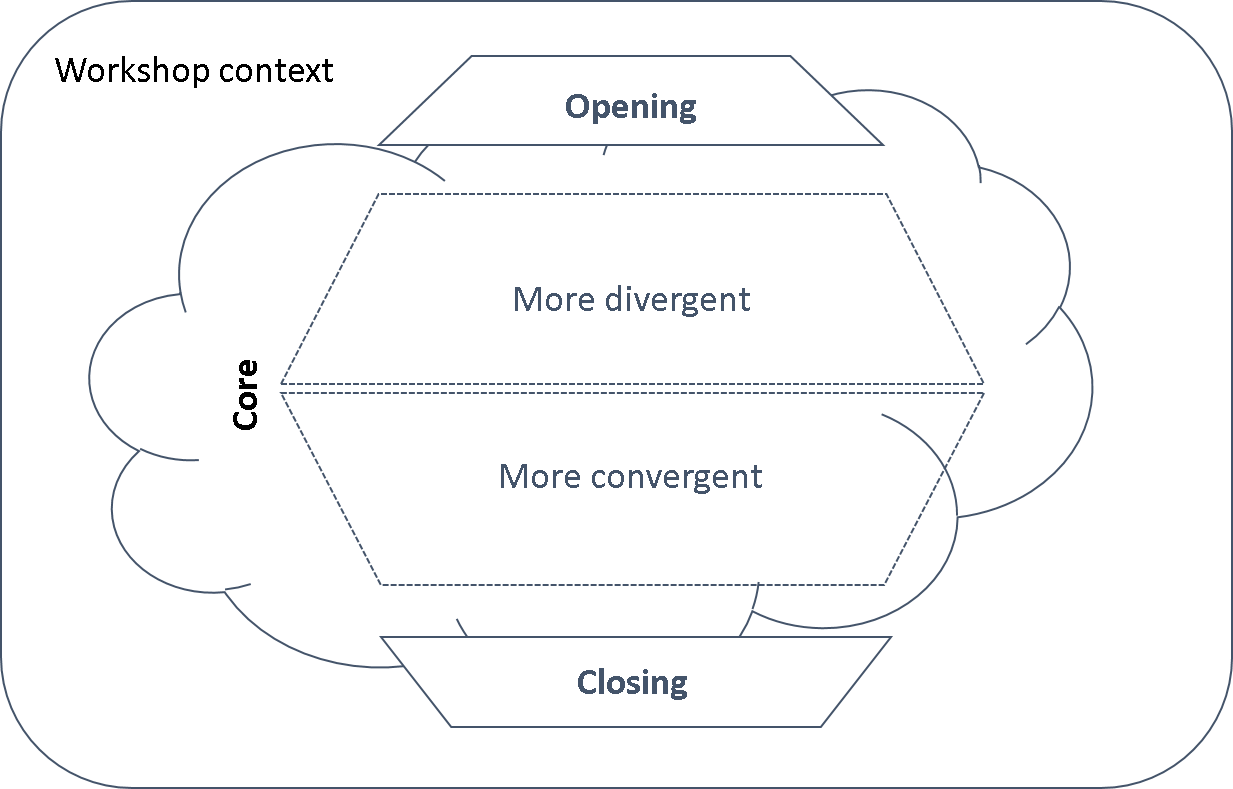
\includegraphics[width=0.8\columnwidth]{figures/workshop-structure.png}
% %     \caption{Workshop structure. Workshops are designed in the context of applied visualization. The workshop opening communicates its intent and purpose. The core supports ideation and exploration, often in cycles of divergent and convergent thinking. The nebulous shape of the core represents the emergent and unpredictable collective creativity. The closing concludes the workshop, establishing next steps for action. \ek{This structure is based on concepts in game storming~\cite{Macanufo2010}, the CPS diamond~\cite{CreativeEducationFoundation2015}, and the consensus workshop~\cite{Stanfield2002}. How should we talk about this?}}
% %     \label{fig:workshop-structure}
% % \end{figure}

% % \subsubsection{Workshop Opening}

% % The workshop opening prepares participants for a productive and creative experience. Effective openings establish an atmosphere conducive to creativity by communicating the workshop purpose, providing agency, and supporting trust.

% % \emph{Purpose}. All of our workshops have started with a short (<5min) introduction \jd{is this the right word? Isn't the point in many ways that we want the assumption that the workshop is passive to be overcome immediately? If so, we could emphasize this. And you do say this later on. So changing this description from `presentation` seems appropriate. Use `Introduction`?} to explain why participants are attending the workshop and what we hope the workshop will create. The opening encourages creativity by encouraging participants to suspend judgment~\cite{Osborn1953}, to commit to the entire workshop~\cite{Hamilton2016}, and to think deeply about concepts~\cite{Sawyer2006}. Telling participants to be creative may not be enough. Successful workshop openings embrace methods that engage participants by providing agency and trust.

% % \emph{Agency}. Effective workshop openings encourage agency, a feeling of ownership, responsibility, and ability to act. Methods that promote agency exhibit multidirectional communication and provide an opportunity for self-expression~\cite{Brooks-Harris1999}. Methods that encourage the one way communication, such as lectures, hinder agency and disengage participants~\cite{Lloyd2011}. Yet, this is a mistake we made in two workshops.

% % \emph{Trust}. Workshops encourage group creativity, the emergent creativity that results from cross-pollination of ideas. Open communication is critically for group creativity and it relies on trust, the confidence that participants place in each other and in the workshop team~\cite{Sawyer2003}. Methods that encourage trust show an intent to listen and demonstrate vulnerability~\cite{Brooks-Harris1999}.
% % \ek{Is there anything else to say about the opening? Maybe 'shake things up' or 'surprise' or 'be playful'}
% % \jd{Probably -- not sure whether this comes here or not, but something like ... This is important that workshop coordinators may deliberately try to `shake things up' a little with exercises that involve surprise or aspects of play. Judgment calls on exactly what is appropriate here are difficult, but we encourage conveners to consider using surprise and play at the outset to establish and encourage agency and trust. Note -- we should also remind ourselves that feedback on whether what we were trying to achieve through these actions will help us make better decisions in the future.}

% % \subsubsection{Workshop Core}

% % After the opening is the workshop core where participants generate, explore, and evaluate a variety of ideas. While there are practically infinite possibilities for the workshop core, reflection on our experience illuminates common concepts that we have found useful for designing workshops: the ideaspace; the visualization, data, analysis and automation context; externalization; connection; and incubation.
% % \jd{Good -- but we need to show how we got there}

% % \emph{Ideaspace.} Methods are characterized \jd{This is very defninitive -- and as we have not proven this as yet I think we need gentler language: `Methods can be characterized...`} by their influence on an ideaspace, the abstract set of all ideas being considered ~\cite{Biskjaer2017,McKenna2014,Osborn1953}. Divergent methods generate ideas and expand the ideaspace. Convergent methods evaluate ideas and winnow the ideaspace. Workshops consist of \jd{Again, I would say -- `Can work well when they consist of ...'} repeated diverge-converge cycles \jd{This is not shown particularly well in Fig 2.}, exploring a broad space of possible ideas before selecting the more promising ones~\cite{CreativeEducationFoundation2015,Osborn1953}. Diverge-converge cycles occur at different scales, between and within methods as workshops start with divergent methods, such as brainstorming to generate ideas followed by grouping those ideas into meaningful clusters~[\ref{wor:arbor}]. Diverge-converge cycles also occur within methods such as workshops brainstorming to generate ideas and then asking participants to highlight the more interesting or important ideas~[\ref{wor:edina}].

% % \emph{Externalization.} Methods are also characterized by the physical artifacts that they produce, in other words, how they encourage or support externalization. This is important to foster creativity as creating a physical representation of an idea starts a feedback loop that forces the idea to evolve~\cite{Sawyer2006}. It is also important for workshop analysis as visualization researchers will eventually make sense of the workshop output. Effective externalization create physical representations of ideas, such as post-it notes, sketches, or other physical representations. Methods without useful artifacts include unstructured group discussion. The externalization also allows methods to be connected into a coherent workshop. 
% % \jd{Communication needs a mention here as `open communication` is mentioned as an aim)}

% % \emph{Connection.} Related to externalization is connection, the way in which methods are connected to form a coherent workshop. Connection promotes revisiting of concepts to discover emergent ideas. Externalization can support connection as output from one method is input to another. For example, by generating ideas on post-it notes and then clustering or ordering those post-it notes. Methods can also be connected implicitly, for example, by asking participants to create new ideas based on previous discussions. 

% % \emph{Incubation.} Providing downtime in a workshop can promote the generation of ideas. More specifically, providing time for ideas to incubate, both through conscious and unconscious thought, is critical for creativity~\cite{Sawyer2006} and should be integrated into workshops. Incubation is supported through passive methods that provide breaks or time to listen without necessarily generating ideas. In shorter workshops, unstructured breaks between methods provide brief periods of incubation~[\ref{wor:lineage}]. In longer workshops, breaks for nutrition and refreshment~[\ref{wor:eon}~,\ref{wor:graffinity},~\ref{wor:cp}] encourage incubation. Reflecting on the impact of incubation on one workshop~[\ref{wor:eon}], a workshop team member described the discussions afforded unstructured lunch: \emph{``Conversation just flowed well! The morning had prompted a lot of ideas and there was a really interesting and diverse discussion over lunch about the subject and possibilities in the area. I expect this was partly also due to the fact that everyone was forced to eat at the neutral venue - lunch was served in a really nice dining area, no decisions had to be made~...~There were no distractions. So we just continued to discuss the topic.''} \ek{Need to condense this quote.}

% % \ek{Is there anything else to say about the workshop core? Maybe that the principles of the workshop opening still apply.}
% % \jd{I'd emphasize the need to continually work to get the balance right -- this is reactive thinking and requires some judgment, but the judgment can be informed by some of the concepts listed here. So -- has there been an opportunity for incubation? Has the planed externalization worked? Where are we with the Ideaspace? Earlier on we talk about (emphasize) flexibility in planning, but this is where the flexibility is used to deliver something that works. So a reminder of that reactive decision-making role would be good here, as would the criteria that we are using to make those decisions.}

% % \subsubsection{Workshop Closing}

% % %% JD -- After the core, the workshop closing concludes the workshop, providing participants with a sense of closure through reflection on their experience and validation of their efforts. The workshop closing is also an effective time to gather feedback from participants.
% % \jd{I find the continual reminders of the order a little jarring -- you could say the following ...}
% % Participants gain closure through reflection on their experience and validation of their efforts. An effective closing can also be a good time to provide some space for incubation and gather considered feedback from participants.
% % \jd{As I mention above, I think we need structured feedback on the process as well as on the subject. We should ask whether and where the things we were trying to foster (agency, purpose, trust communication, etc.) were experienced (strongly?) and where they were not}

% % \emph{Reflection.} Reflective methods ask participants to analyze their experience in the workshop. A common example is to ask participants about interesting ideas from the day.
% % \jd{Is this a good example of reflection? It seems a bit obvious? This sounds like `remembering`. To me, reflection is more about relating experiences to a benchmark -- such as expectations, so asking specific questions about how the ideas, or the process, or the communication compare to other experiences makes sense. What do participants `reflect` their thinking into / onto? E.g. the quote in para 1 reflects on the workshop vs. a regular team meeting -- `more team progress in a day than we make in a year of lab meetings`. I think we could give some guidance on the kinds of reflection that might work here -- what surprised you, where did we not make progress, etc.
% % Actually, I have noticed now that you do this quite well in \subsubsection{Workshop Closing} -- so this should be easy to adapt here.} 
% % Reflection provides information for the workshop team about what participants found more interesting, guiding the analysis of workshop results. The reflection can also give participants confidence that their time was used effectively as ideas have often evolved throughout the day.
% % \jd{This is about reflecting current knowledge state back to initial knowledge state to reveal difference -- good}

% % \emph{Validation.} The workshop closing is an opportunity to provide participants with a sense of validation. This includes thanking participants for their participation in the workshop.  It is also important to communicate the next steps of the project, to validate that participant’s energy will influence the direction of the collaboration~\cite{Hamilton2016}.
% % \jd{This feels weak -- `Say thank-you`. Is there more here? What is important?}

% % \emph{Feedback.} The closing is also a time to ask for feedback on the workshop. This includes communicating surveys to participants to asking for feedback through other methods. \ek{what else can we say about feedback?}
% % \jd{I think this is weak too -- see above and other comments. I think we need feedback on the contents of the workshop -- which ideas float, following some incubation and some reflection is there anything else to add? Do we have other ideas? Can we synthesize ideas? --- but also on the workshop itself and this is where I think we need structured feedback on whether our intentions were achieved (trust, purpose, agency, etc.). We did this to an extent at E.ON, asking whether participants felt agency as this was what we were trying enable them to achieve.}

% % Following the workshop, ideas and artifacts from it are analyzed. The analysis drives forward the visualization project by identifying areas for future work, exposing shared user needs, and establishing criteria for evaluating ideas.
% % \jd{I know why this is here, but without a reminder that we will actually be giving some guidance in 6.4 this feels a bit obvious. We almost need to say something here like ... `effective analysis will be dependent upon what has been recorded during the workshop so making good judgments on analytical methods post-workshop is absolutely key`. This is also obvious and boring but at lest it reminds us of the need to be adaptive?
% % }

% % \subsection{Illustrative Example Workshop}

% % \begin{figure*}[t]
% %     \centering
% %     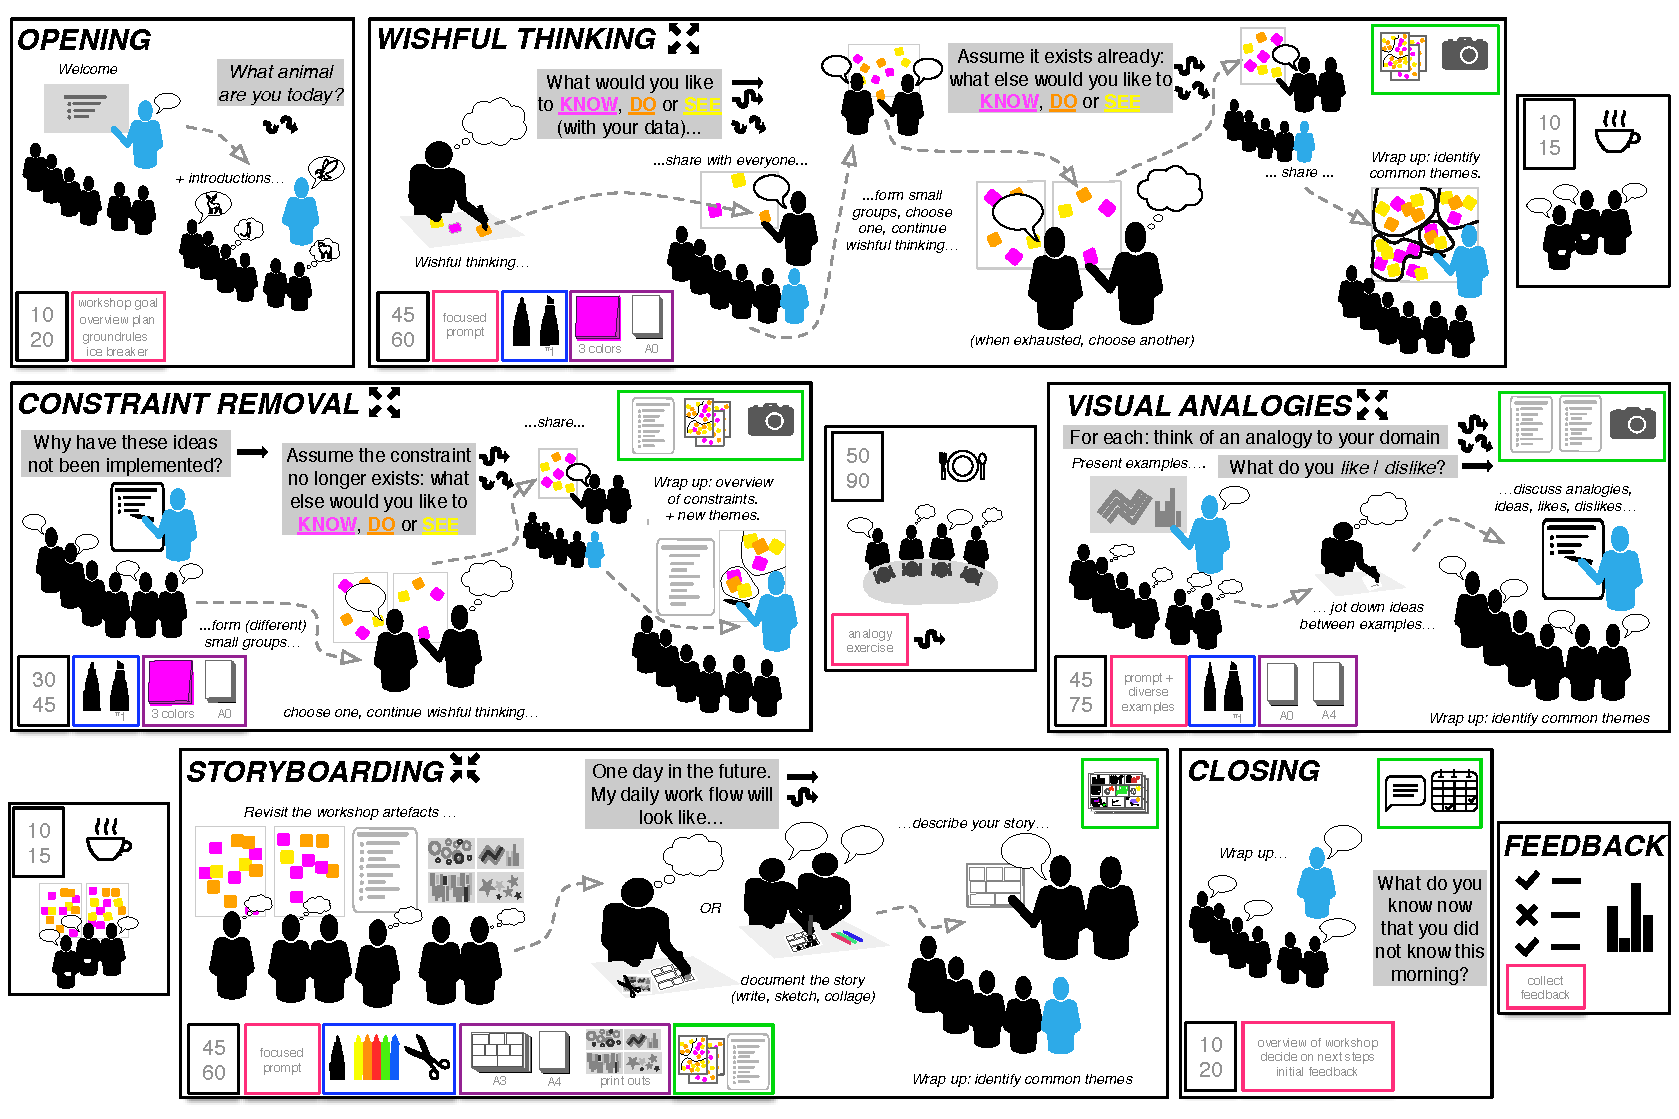
\includegraphics[width=0.8\textwidth]{figures/example-workshop.pdf}
% %     \caption{A validated full day requirements workshop that illustrates the workshop structure and serves as a starting point for future workshops. The opening establishes a creative atmosphere, encouraging trust and agency. The core allows for exploration of ideas. The closing summarizes, validates, and concludes the workshop. \ek{Something to think about: how can we put this in the same style as Fig.~\ref{fig:workshop-structure}?}}
% %     \label{fig:example-workshop}
% % \end{figure*}

% % We illustrate the workshop structure with a full day workshop, shown in Fig.~\ref{fig:example-workshop}, that has been validated in design studies with energy analysts~[\ref{wor:eon}], constraint programmers~[\ref{wor:cp}], and neuroscientists~[\ref{wor:graffinity}]. This subsection examines the intent of methods used during the opening, the core, and closing at a high level of abstraction. The next subsection unpacks the nuanced differences between the projects where we used this workshop. Together, they provide a starting point \jd{Is this right - or are they an example of a design that meets our criteria?} for future workshops. But ultimately, this is one sample of a practically infinite workshop design space.

% % \jd{OK, but we need to be clearer about why it is useful. Showing how it addresses the criteria (converge / diverge; adapt; provide agency; engender trust; etc). I'd also emphasize that this has been adapted with experience as well as `validated' -- to me that is valid validation! As I said above on `feedback' I think we need to think about how we adapt these things with experience as we learn -- we need to acquire feedback on the criteria (see above) that we are aiming to achieve and show that we have made changes in light of this and our own reflection.} 
% % \jd{So (like any graphic or system we might design) this is one in a gazillion, but it is one that has some characteristics that might guide others.}

% % \subsubsection{Workshop Opening}

% % The workshop opening consists of a short presentation and introduction method. \jd{Another statement that is too definitive for me. What is this about? We already know that workshops should start with this as we read this in section 4. So I am not sure what the opening two sentences here add?} The presentation communicates the purpose of the workshop and articulates how the researcher will use the workshop outputs to guide the collaboration. The presentation also establishes guidelines for encouraging group creativity. Example guidelines used in a previous workshop~[\ref{wor:eon}] are: 
% % \begin{itemize}[noitemsep,nolistsep]
% % \item all ideas are valid --- record them;
% % \item let everyone have their say; 
% % \item be supportive of others; 
% % \item instead of criticizing, create additional ideas;
% % \item think 'possibility' – not implementation; 
% % \item speak in headlines and follow-up with detail; and 
% % \item switch off all electronic devices.
% % \end{itemize}

% % Next, an \emph{Analogy Introduction} asks the workshop team and participants introduce themselves through analogy, such as \emph{``What animal are you today?''} This method provides agency through self-expression. It promotes trust by encouraging the display of vulnerability and if participants are given time to respond in turn it ensures inclusivity from the outset. Reflection on this experience reveals~[\ref{wor:eon}]:  {\it ''the animal introductions required some audacity on the part of our facilitator...it seemed useful preparation for future exercises in initially putting all participants on an equal footing.``}
% % \jd{I also think that the analogy introduction should be used explicitly as a means of testing / practicing the guidelines. It's a test-bed or pilot for what follows.}

% % \subsubsection{Workshop Core}

% % The workshop core starts with a divergent active method \emph{Wishful Thinking}, that elicits participants’ aspirations for visualization software. Prompted with a scenario in their domain, participants respond to the following three questions on post-it notes: \emph{What would you like to be able to see? What would you like to be able to know? What would you like to be able to do?} Participants share ideas through group discussion before generating more ideas in small groups.

% % The ideas generated in \emph{Wishful Thinking} cascade through the workshop as they are input to the next divergent, active method \emph{Barrier Removal} that asks participants to identify and record barriers in the way of their aspirations. These barriers are then \emph{`removed'} by imagining what would be possible if the barrier no longer existed. These ideas are recorded on post-it notes, following the same \emph{know/see/do} prompts. This method promotes divergent thinking as participants are asked to generate additional ideas. Next, time for lunch is provided to allow for incubation and unstructured discussion.  

% % \jd{I would put a reflective session here following incubation over lunch -- ``Did anybody think of anything interesting over lunch?''!}

% % After lunch, the participants return to a divergent, passive method, \emph{Visualization Analogies}, where participants are shown a variety of visualizations and record ideas about how the visualization may apply to their domain. \jd{LIkes / dislikes are mentioned explicitly in the figure but no here} This method is similar to visualization awareness workshops~\cite{Koh2011}. It engages participants, allowing them to think creatively about their problem domain with a curated set of graphics and develop requirements by example.

% % After a short break, a convergent method, \emph{Storyboarding}, is used to winnow the ideas into coherent narratives as participants depict `a day in their life' while imagining the impact of topics from the workshop. \emph{Storyboarding} is implicitly connected to the previous methods.
% % \jd{It would be good to say a little more about outputs and rationale here -- I don't have too much confidence in storyboarding, others may want to lead on this!}

% % \subsubsection{Workshop Closing}

% % The workshop concludes with a reflective closing method where participants are asked \emph{``what do you know now that you did not know this morning?''} Because this question is intended to start a discussion, it requires participants prioritize their thoughts to talk about the more interesting ideas. Recording this discussion provides important cues for the workshop team to jump-start their analysis.

% % \jd{It does feel a little strange that we have the (design of the) example workshop before we have read through ``Design Considerations''}

% % \subsection{Workshop Design Considerations}

% % This section describes differences between the example workshops \jd{Which ones - the illustrative example in \subsection{Illustrative Example Workshop} or the full set under consideration here?''} in action, revealing the subtleties of workshop design and execution. We use these differences as a springboard for examining high-level workshop design considerations.

% % \subsubsection{Example Workshop in Action}

% % The three projects that used the example workshop exhibited differences as we we tailored the workshop to the specific project context, to our experience as visualization researchers, and to our comfort level facilitating workshop discussions.

% % \emph{Context.} We adapted the workshop methods to the context and desired outcomes of each project. We tailored the \emph{Wishful Thinking} method by adjusting the prompt for each of our three projects. Our collaboration with energy analysts focused on long term goals for a forward-thinking smarthome program and we asked participants to: \reviseme{\emph{“think about aspirations for the Smart Home programme … ‘What would you like to know?’, ‘What would you like to be able to do?’ and ‘What would you like to see?’”}} In contrast, working with constraint programmers examined shorter-term goals and concrete analysis tasks: \emph{“Your program does not execute as expected…[what would you like to know/see/do]?”} A similar concrete aspect was used in the neuroscience workshop: \emph{“Suppose you are analyzing a connectome, [what would you like to know/see/do?]”} This workshop also used screenshots of existing tools to stimulate ideas. Although the difference in wording may be subtle, the connection between methods means that these ideas propagate through the workshop. It is important to tailor the methods to the appropriate context. 

% % \emph{Experience.} We adapted the workshop methods to reflect our experience, knowledge, and style. In the \emph{Visualization Analogies} method, we presented different visualizations in each workshop. Reflecting on our experience revealed that we selected visualizations that we could talk about with confidence, to establish trust by demonstrating our credibility. We also identified common themes of how to select visualizations, including a mix of seemingly unrelated visualizations (to promote divergent thinking), visualizations that you created (to show authority and credibility), visualizations that you did not create (to show knowledge of the field), older visualizations (to show depth of knowledge), and playful visualizations (to support engagement). The emphasis on analogy in this method has generated many interesting discussions, such as \emph{``what does it mean for legends to move?''}~[\ref{wor:edina}], \emph{``what does it mean for energy to flow?''}~[\ref{wor:eon}], and \emph{``what does it mean for neurons to rhyme?''}~[\ref{wor:graffinity}]. 
% % \emph{One thing we want to emphasize is that by diverging and then converging we often converge on something that was beyond the bounds of our original Ideaspace. This is important. It's also one of the reasons I don't like Fig.~\ref{fig:workshop-structure} much. It looks here as though the divergence and convergence gets you back to where you started. But really you have moved -the process has shifted you somewhere. It also looks like an exploding polystyrene takeaway food package -- but I can probably live with that. Just.}

% % \emph{Execution.} Although workshops can plan to use the same methods, they will follow different execution processes depending on the experience of the workshop team or feedback from the workshop participants. An example of this is how we used the \emph{Wishful Thinking} method with different processes (shown in Fig.~\ref{fig:wishful-thinking-process}). One process involved individual ideation, large group discussion, and then small group ideation. The other process relied on hierarchical aggregation of ideas, moving from individual ideation, to small group ideation, to large group discussion. Execution processes can also differ in how participants form small groups for ideation or discussion. We have \emph{shuffled} participants into groups based on a variety of factors, including by their organization (visualization research vs domain specialist), seniority, gender, research focus, or by chance. Although it is impossible to prescribe the most effective course of execution, it is important to recognize that execution will vary between workshops based on many factors. 
% % \jd{This section would be better if the factors, and our responses to them, were more clearly stated}.

% % \subsubsection{Design Considerations}

% % \begin{figure}[t]
% %     \centering
% %     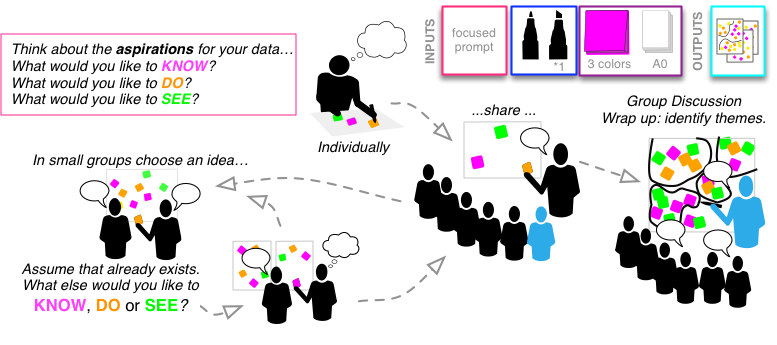
\includegraphics[width=\columnwidth]{figures/wishful-thinking-process}
% %     \caption{\ek{Placeholder} Workshops that use the same methods will be executed with different processes, such as the process of \emph{Wishful Thinking} shown here. In one case (top), individual ideation is followed by large group discussion that segues to small group ideation and discussion [\ref{wor:eon},~\ref{wor:cp}]. In the other case (bottom), individual ideation is followed by hierarchical discussion, from small group to large group discussion [\ref{wor:graffinity}]. We illustrate this difference to encourage thinking about which method may be more appropriate.}
% %     \label{fig:wishful-thinking-process}
% % \end{figure}

% % \jd{But in Fig.~\ref{fig:wishful-thinking-process} we don;t say anything about how we know which is most appropriate - what are the criteria?}

% % We introduced the workshop structure and illustrative example to provide a starting point in the workshop design space. This subsection describes considerations for exploring that design space. It emphasizes that there are limitless workshop possibilities. It identifies criteria for evaluating workshops based on how they support creativity. It summarizes resources that may be useful for selecting methods, and describes how methods can be tailored for visualization workshops.

% % \emph{Limitless Possibilities.} The validated example represents a minority of our experience as all other workshops relied on different structure. True, a set of these workshops were condensed versions of the example~[\ref{wor:lineage},~\ref{wor:updb}]. But the other workshops used entirely different methods that seemed appropriate for the workshop context. Working with defense analysts, we used methods that identified surrogate data to use in place of classified human terrain reports~[\ref{wor:htva}]. Working with biologists, we explored key aims for a grant proposal instead of requirements for visualization software~[\ref{wor:arbor}]. Working with GIS researchers, we identified key themes to explore the design space of interactive legends through brainstorming and prioritization [\ref{wor:edina}]. A summary of the methods used in each workshop is included in our supplemental material. These differences illustrate that workshops will look different depending on the project and the project goals. 

% % \emph{Creativity Support.} Framing workshops as \emph{creativity support tools} provides valuable criteria for their design and evaluation. Shneiderman et al.~\cite{Shneiderman2005} proposed the following guidelines for creativity support software, but the same principles apply to effective workshops:
% % \begin{itemize}[noitemsep,nolistsep]
% % \item  \emph{Support collaboration and communication} --- workshops support communication by encouraging group work and explicitly externalizing ideas.
% % \item  \emph{Provide low barriers, high ceilings, wide walls} --- workshops encourage exploration through easy-to-use methods and undefined stopping conditions.
% % \item  \emph{Make it as simple as possible} --- workshops focus participant energy on the ideas, instead of understanding the method.
% % \item  \emph{Invent things that you want to use yourself} --- workshops use methods that are fun and engaging.
% % \item \emph{Support many paths and many styles} --- workshops support the different styles and preferences of participants.
% % \end{itemize}
% % Combining these guidelines with the workshop structure provide a foundation for selecting methods for creativity workshops.
% % \jd{Sure, but we are a little shor of examples that show that we have used these criteria in our selection}.

% % \emph{Method Resources.} Workshop methods can be selected from a plethora of resources. Particularly useful resources that we have used are from the fields of visualization, design, and business. McKenna et al.~\cite{McKenna2014} provide 100 exemplar methods relevant for visualization researchers, but these methods may need to be adapted to a workshop setting. Kumar~\cite{Kumar2012} describes 101 product design methods useful in a business setting. Gray et al.~\cite{Macanufo2010} describe \emph{games}, methods that encourage creative thinking and can be chained together into workshops. The seminal work of the Creative Problem Solving Foundation~\cite{CreativeEducationFoundation2015,Osborn1953}, Synectics~\cite{Gordon1961}, and Lateral Thinking~\cite{DeBono1983} may also be useful for thinking about workshop design. All but one of these resources were targeted for domains outside of visualization and the methods should be adapted for visualization design.

% % \emph{Method Adaptation.} We adapt methods to visualization by injecting vocabulary, prompts, or other materials that explicitly reference domain problems, data analysis, automation, and visualizations. One example of this is the \emph{Wishful Thinking} method. This is a visualization-specific form of \emph{Aspirations Thinking}~\cite{McFadzean1998b} adapted by prompting participants to think about their data analysis and by using visual language. Another example is the use of \emph{Visualization Analogies}, which resembles analogy-based creativity methods~\cite{Gordon1961} but has been customized to excite participants about visualization while demonstrating the workshop team's breadth of visualization knowledge. We include these examples to inspire the design of more creativity methods that explicitly explore the relevance and role of visualization, data, analysis, or automation. 

% % \emph{Mutual Learning.} In addition to exploring the importance of data, analysis, and visualization, the workshops of creativity methods should promote mutual learning of visualization researchers and domain collaborators. Examples of this abound in our experience --- \emph{Wishful Thinking} creates artifacts that teach visualization researchers about the aspirations of the domain analysts, and \emph{Visualization Awareness} can demonstrate important concepts of visualization design such as multiple linked views, overview-to-details, and specialized visual encodings. Methods can promote mutual learning by exploring the state of the domain, by encouraging collaborators to present scenarios about their domain~[\ref{wor:htva}] or asking about current successes and problems of existing tools~[\ref{wor:edina}].

% % \emph{Limitations of Design.} The concepts in this section are a starting point for designing workshops. They are thinking tools and resources for describing methods, but they do not account for the complexities of human thought~\cite{Sawyer2006}, the emergent nature of group creativity~\cite{Sawyer2003}, nor the serendipitous interactions that workshops support~\cite{Brooks-Harris1999}.  Ultimately workshop design involves working out which of a set of methods we might use and what effect they might have on the workshop. But the workshop execution requires flexibility in terms of execution process and in light of unpredictable reactions that occur during the workshop. Both the design and execution should be considered in the context of the entire applied visualization collaboration. Recommendations for the entire process, from deciding to using a workshop to designing the workshop methods, executing the methods, and analyzing the results are described next.

% % \jd{I think we are saying that you need a design structure and flexibility within this. So planning that offers different implementation pathways makes sense to me. This may be what you are about to show next ..?}